%% sage_latex_guidelines.tex V1.10, 24 June 2016

\documentclass[Afour,sagev,times]{sagej} %sageh

% customizations
\usepackage[super]{nth}
\usepackage[inline]{enumitem}
\usepackage{moreenum}
\usepackage{tabulary}
\usepackage{tabu}
\usepackage{booktabs}
\usepackage{array}
\usepackage[super]{nth}
\usepackage{listings}
\usepackage{float}
\usepackage[mode=buildnew]{standalone}
\usepackage{tikz}
\usepackage{upquote}
\usepackage{graphicx}
\usepackage{epstopdf}
\usepackage{tabularx}
\usepackage{import} %\usepackage{newclude}
\newcolumntype{Y}{>{\raggedright\arraybackslash}X}
\newcommand{\ra}[1]{\renewcommand{\arraystretch}{#1}}

% special characters
\usepackage{gensymb}
\usepackage{amssymb}
\usepackage{pifont}
\newcommand{\cmark}{\ding{51}}
\newcommand{\xmark}{\ding{55}}

% sage packages and commands
\usepackage{moreverb}
\usepackage[hyphens]{url}
\usepackage[colorlinks,bookmarksopen,bookmarksnumbered,citecolor=red,urlcolor=red]{hyperref}
\newcommand\BibTeX{{\rmfamily B\kern-.05em \textsc{i\kern-.025em b}\kern-.08em
T\kern-.1667em\lower.7ex\hbox{E}\kern-.125emX}}


% ---------------------------- METADATA ---------------------------- 

\def\volumeyear{2017}
\begin{document}
\runninghead{Harmon et~al.}
\title{Tangible topographic modeling for landscape architects}
\author{Brendan Harmon\affilnum{1,2}, Anna Petrasova\affilnum{2}, Vaclav Petras\affilnum{2}, Helena Mitasova\affilnum{2}, and Ross Meentemeyer\affilnum{2}}
\affiliation{\affilnum{1}Robert Reich School of Landscape Architecture, Louisiana State University, USA\\
\affilnum{2}Center for Geospatial Analytics, North Carolina State University, USA}
\corrauth{Brendan A Harmon, 
Robert Reich School of Landscape Architecture,
Louisiana State University,
Baton Rouge, LA 70803, USA.}
\email{brendan.harmon@gmail.com}

% ---------------------------- ABSTRACT ---------------------------- 

\begin{abstract}
We present Tangible Landscape -- a technology for rapidly and intuitively designing landscapes informed by geospatial modeling, analysis, and simulation. Tangible Landscape is a tangible interface powered by a geographic information system that gives 3D spatial data an interactive, physical form so that users can naturally sense and shape it. It couples a physical and a digital model of a landscape through a real-time cycle of physical manipulation, 3D scanning, spatial computation, and projected feedback. Natural 3D sketching and real-time analytical feedback should aid landscape architects in the design of high performance landscapes that account for physical and ecological processes. We conducted a series of studies to assess the effectiveness of tangible modeling for landscape architects. Landscape architecture students, academics, and professionals were given a series of fundamental landscape design tasks -- topographic modeling, cut-and-fill analysis, and water flow modeling. Their performance was assessed using qualitative and quantitative methods including interviews, raster statistics, morphometric analyses, and geospatial simulation. With tangible modeling participants built more accurate models that better represented morphological features than they did with either digital or analog modeling. When tangibly modeling they worked in a rapid, iterative process informed by real-time geospatial analytics and simulations. With the aid of real-time simulations they were able to quickly understand and then manipulate how complex topography controls the flow of water.
\end{abstract}

\keywords{Human-computer interaction, tangible interfaces, tangible interaction,
landscape architecture, performance, geospatial modeling, 
topographic modeling, hydrological modeling}

\maketitle

% ---------------------------- INTRO ---------------------------- 

\section{Introduction}

% performance
In performance-based landscape architecture 
-- like in performative architecture \cite{Kolarevic2005} --
the functional performance of the landscape drives the design.
A landscape's performance 
can be quantified through factors such as
ecosystem services, risk of natural hazards, plant health, 
hydrology, geomorphology, and biodiversity. 
% strategies
Strategies for performance-based landscape architecture include
monitoring and assessing how well landscapes function
after they have been built, \cite{Yang2016}
analyzing how landscapes function before designing interventions,
testing alternatives through adaptive experiments,
adaptively managing landscapes as they change, 
and comparing alternative future scenarios 
based on quantitative metrics. \cite{Lovell2015}
% computation
While parametric modeling informed by computational analysis 
can play a generative, form-finding role 
in performative architecture, 
performance-based landscape architecture 
currently relies largely upon research and assessment.
Since landscapes are shaped by physical and ecological processes,
geospatial modeling and simulation could play a truly generative role 
in the design of high performance landscapes.
%
For geospatial computation to 
play such a generative role
it would need to be an integral part 
of the creative design process.

% GIS and CAD in landscape architecture
Landscape architects use 
geographic information systems (GIS) to map and analyze landscapes
and computer aided design (CAD) software
to computationally represent and design landscapes.
While GIS can quantitatively model, analyze, simulate, and visualize 
complex spatial and temporal phenomena,
these systems can be unintuitive, 
challenging to use, and creatively constraining
due to the complexity of the software, 
the complex workflows, 
and the limited modes of interaction and visualization. 
\cite{Ratti2004}
Due to the complex, time consuming workflows 
needed to link geospatial analysis with computer aided design, 
GIS tends to play a limited, 
often preliminary role in the creative design process.
While GIS has been used extensively in landscape planning 
to model scenarios, \cite{Steinitz2004,Baker2004,Steinitz2012}
in landscape architecture
it is primarily used for preliminary research and mapping.
If, however, geospatial analysis, modeling, and simulation
could be seamlessly integrated into the creative design process 
then designers could rapidly develop design ideas
while quantitatively testing them. 
In such a rapid, fluid creative process
the rigorous testing of design concepts 
with quantitative measures of performance 
could drive the development of new concepts.

% tangibles
When using a graphical user interface (GUI) 
-- the paradigmatic mode of interaction for both CAD and GIS --  
intention is translated from physical input 
using devices like a mouse and keyboard 
to digital data rendered visually as text and graphics. 
Positing that graphical interaction is unintuitive
because of this disconnect between 
intention, physical action, and purely visual feedback,
researchers have been developing tangible user interfaces 
to give digital data interactive physical form. 
\cite{Dourish2001,Ishii2008} 
Theoretically tangible interfaces should embody cognition 
-- grounding higher cognitive processes in bodily experience --
by enabling users to kinaesthetically sense and interact with digital data.
\cite{Kirsh2013}
Tangible, embodied interaction should be highly intuitive 
because it uses existing motor schemas,  
offloads cognitive work onto the body,
and seamlessly connects intention, action, and feedback.

% tangibles for landscape architecture
The MIT Media Lab developed two prototypes 
-- Illuminating Clay and SandScape -- 
that coupled a physical and digital model of a landscape
through a cycle of 3D scanning, geospatial computation, and projection
to combine the affordances of intuitive sculpting by hand
with quantitative geospatial analysis. \cite{Piper2002a}
These systems were designed to 
`streamline the landscape design process 
and result in a more effective use of GIS, 
especially when distributed decision-making and discussion 
with non-experts are involved.' \cite{Ratti2004}
Recent advances in sensors and computer vision
have fueled the development of 
systems for tangibly modeling landscapes such as 
Efecto Mariposa, \cite{Vivo2011}
the Augmented Reality Sandbox, 
\cite{Kreylos2012,ARsandbox}
Sedimachine, \cite{Cantrell2014} and
the Rapid Landscape Prototyping Machine. \cite{Robinson2014}

\subsection{Tangible Landscape}
Inspired by Illuminating Clay, 
the Tangible Geospatial Modeling System, 
\cite{Mitasova2006,Tateosian2010} 
and the Augmented Reality Sandbox, 
we have develop Tangible Landscape 
-- a tangible interface for geospatial modeling
powered by an open source GIS. \cite{Petrasova2015}
With Tangible Landscape
designers can sculpt a terrain model in polymeric sand
and can digitize points, areas, or volumes by placing 
color-coded markers, patches of felt, or building blocks. 
These interactions are captured by a Kinect sensor, 
processed in GRASS GIS, 
and the resulting geospatial computations
are projected back onto the physical model, 
all in real-time (Fig.~\ref{fig:system_diagram}).
The geospatial data can also be automatically
3D modeled and rendered in Blender 
on a monitor or head-mounted display
so that designers can 
immersively explore different views. \cite{Tabrizian2016}
For example
as users sculpt topography,
simulated water flow can be projected back onto the model in real-time
so that they understand how they are affecting 
physical processes in landscape.
Then as they create planting areas 
with colored push-pins or patches of felt,
the trees can be rendered in 3D on a display
(Table~\ref{table:tl_demo}). 

Tangible Landscape is unique since it powered by a GIS
with extensive libraries for geospatial computation
and has a wide range of real-time interactions including 
3D sculpting, 3D sketching, color recognition, and object recognition.
Given its versatility there are many possible design applications
including terrain modeling, hydrological modeling, erosion control, 
flood prevention, trail planning, viewshed analysis, solar analysis, 
and planting design. 

\begin{figure}
    \begin{center}
        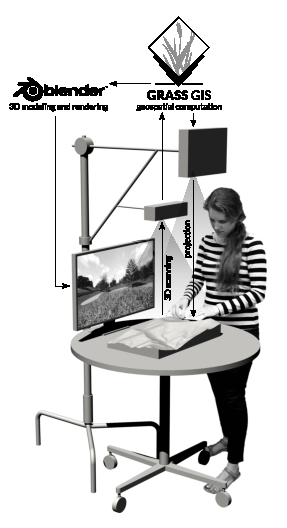
\includegraphics[width=0.45\textwidth]{images/diagrams/rendered_diagram_2.pdf}
        \caption{Tangible Landscape: a real-time cycle of 3D scanning, geospatial computation and 3D modeling, and projection and 3D rendering.}
        \label{fig:system_diagram}
    \end{center}
\end{figure}

%\begin{table*}
%\caption{Collaboratively sculpting topography to create lakes, 
%drawing trees with a laser pointer, and visualizing with 3D renderings.}
%\ra{1.3}
%\begin{tabular}{m{0.49\textwidth} m{0.49\textwidth}}
%\toprule
%\multicolumn{1}{c}{Sculpting}  & \multicolumn{1}{c}{Drawing and visualization}\\
%\midrule
%%
%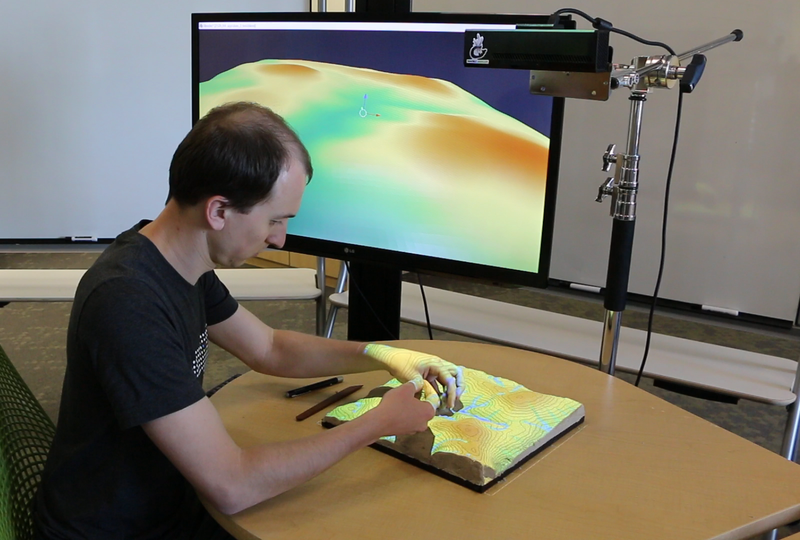
\includegraphics[width=0.49\textwidth]{images/immersive/sculpting_lakes_2.png} &
%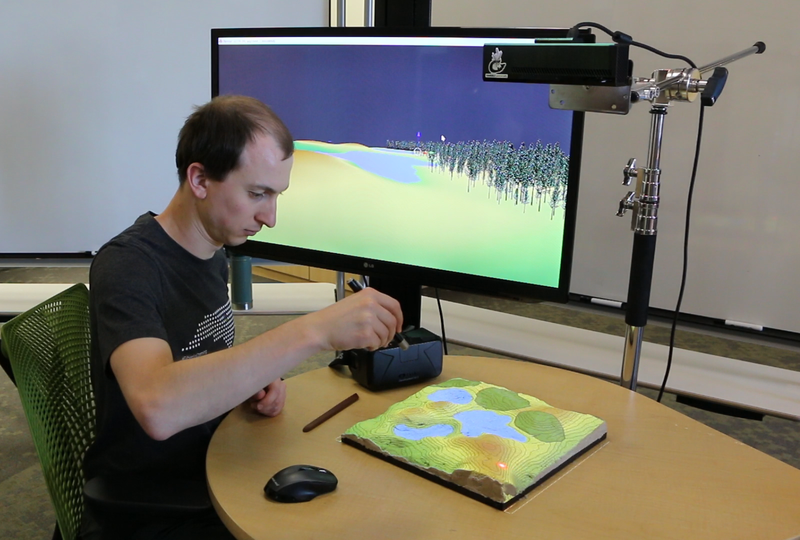
\includegraphics[width=0.49\textwidth]{images/immersive/drawing_trees_1.png}\\
%%
%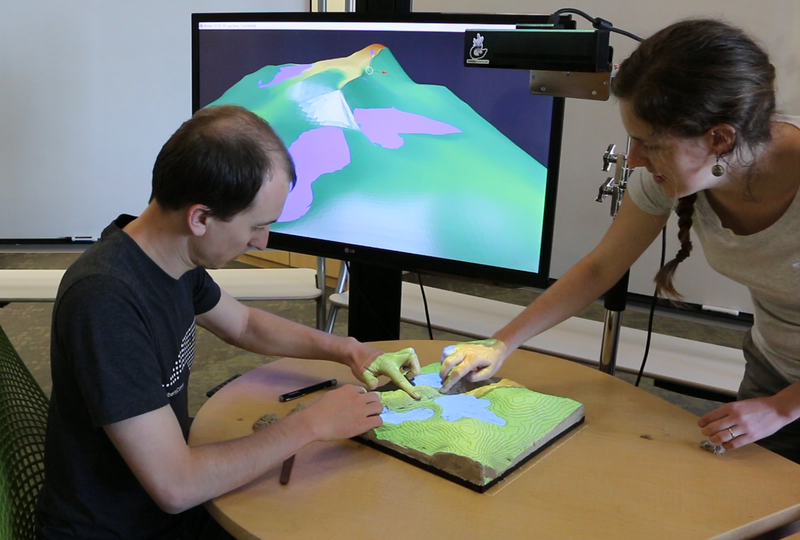
\includegraphics[width=0.49\textwidth]{images/immersive/sculpting_landforms_2.png} &
%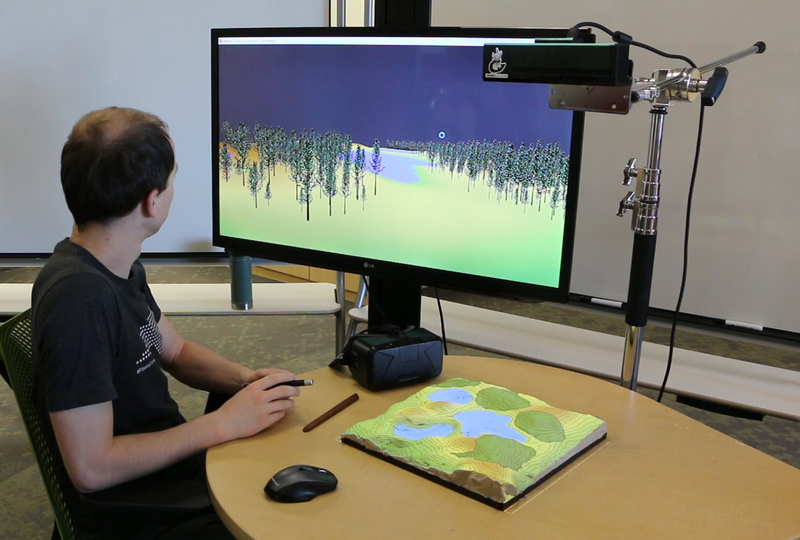
\includegraphics[width=0.49\textwidth]{images/immersive/drawing_trees_2.png}\\
%%
%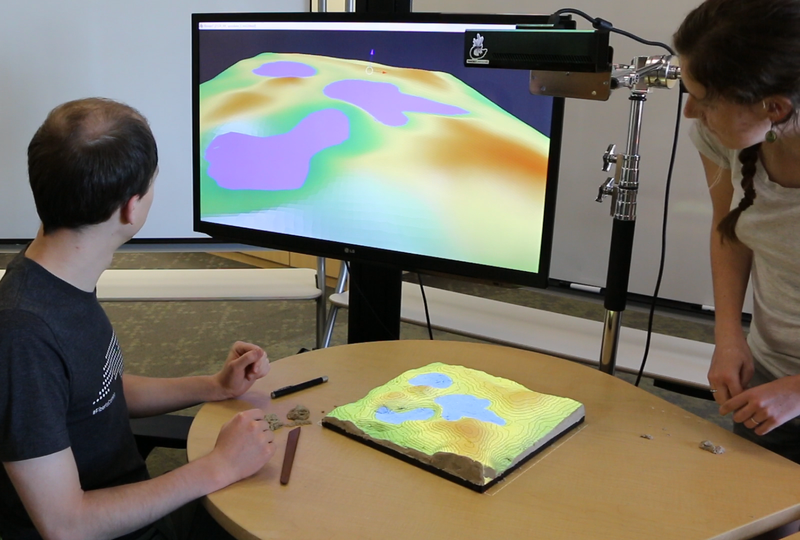
\includegraphics[width=0.49\textwidth]{images/immersive/sculpting_landforms_3.png} &
%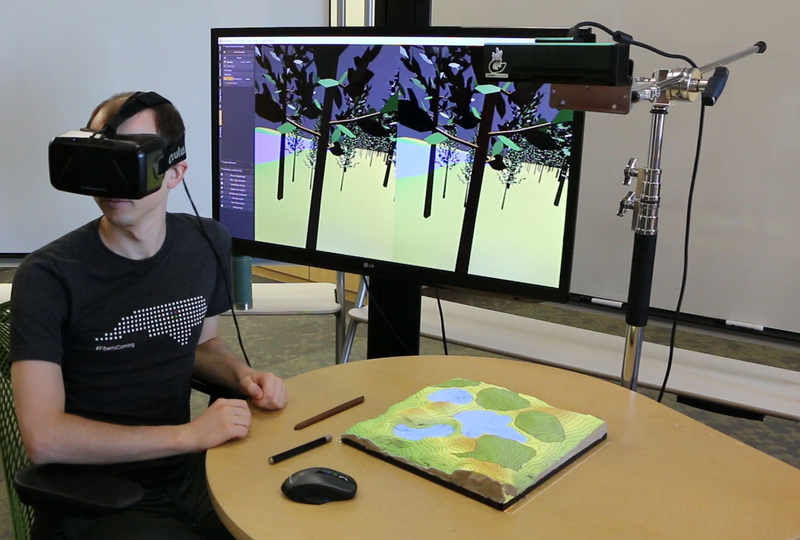
\includegraphics[width=0.49\textwidth]{images/immersive/trees_with_oculus_1.png}\\
%%
%\bottomrule
%\end{tabular}
%\label{table:tl_demo} 
%\end{table*}

\begin{table*}
\caption{Sculpting topography
to create lakes, 
planting trees with felt and push-pins, 
and exploring views. %with Tangible Landscape.
Source: \cite{Tabrizian2017}}
\ra{1.3}
\begin{tabular}{m{0.49\textwidth} m{0.49\textwidth}}
\toprule
\multicolumn{1}{c}{Sculpting}  & \multicolumn{1}{c}{3D planting and visualization}\\
\midrule
%
\includegraphics[width=0.49\textwidth]{images/3d_planting/initial_conditions.jpg} &
\includegraphics[width=0.49\textwidth]{images/3d_planting/planting_4.jpg}\\
%
\includegraphics[width=0.49\textwidth]{images/3d_planting/sculpting_4.jpg} &
\includegraphics[width=0.49\textwidth]{images/3d_planting/specimen_planting_3.jpg}\\
%
\includegraphics[width=0.49\textwidth]{images/3d_planting/view_landform_1.jpg} &
\includegraphics[width=0.49\textwidth]{images/3d_planting/view_specimen_planting_6.jpg}\\
%
\bottomrule
\end{tabular}
\label{table:tl_demo} 
\end{table*}

\subsection{Research objectives}
The aim of this research was to test whether
sandbox-style tangibles could be an effective tool
for landscape design. 
%
Our research objectives were 
to assess how well landscape architects could:
\begin{enumerate*}[label=\alph*),font=\itshape]
\item model topography, 
\item analyze cut-and-fill, 
\item and model water flow
\end{enumerate*}
using a sandbox-style tangible interface for landscape modeling.
%
In order to assess the effectiveness 
of tangible modeling for landscape architects 
we conducted a series of user studies
assessing how well participants performed
these basic landscape design tasks 
%-- topographic modeling, cut-and-fill analysis, and water flow modeling --
using Tangible Landscape.

There have been very few 
case studies, \cite{Ishii2002,Tateosian2010,Petrasova2015}
qualitative user studies, 
\cite{Shamonsky2003,Woods2016}
and quantitative studies \cite{Schmidt-daly2016b}
about sandbox-style tangibles.
%
While the quantitative study by
Schmidt-Daly et al.~\cite{Schmidt-daly2016b} 
assessed both learning and task performance,
it did not assess the unique and most important 
affordance of sandbox-style tangibles --
freeform 3D sculpting. 
% 
Sandbox-stye tangibles uniquely afford
the ability to sculpt digitally augmented, 
freeform 3D volumes
with ones bare hands. 
%
While there are standard, validated
pre- and post-tests for assessing learning
in human-computer interaction,
methods for assessing task performance 
are specific to the task
(see for example Cuendet et al.~\cite{Cuendet2012}).
%
Furthermore,
in a pilot study we found that the only 
validated test for reading topography -- the
Topographic Map Assessment test
\cite{Newcombe2015} --
was too easy for landscape architects.
%
Therefore, we developed 
new, spatially-explicit methods
for assessing performance
in freeform 3D modeling tasks.
%
We used raster statistics, 
morphometric analyses, and geospatial simulation
to assess the spatial accuracy, pattern and distribution
of the results for each task. 

% ---------------------------- TOPOGRAPHIC ---------------------------- 

\section{Topographic modeling}
%
One of the primary tasks of landscape architects is to design earthworks.
\cite{Petschek2008,Strom2013}
% topographic data
Landscape architects work with topographic models 
derived from data collected by field surveys, airborne lidar, 
or photogrammetry with unmanned aerial systems.
% designing landforms
They design new landforms 
using analog methods -- such as 
drawing contours maps by hand and
hand sculpting physical topographic models in clay --
and digital methods -- such as 
drawing digital contour maps in CAD and
digitally sculpting surfaces in 3D modeling software. 
% analog
Analog methods for topographic modeling are typically used 
in the early, conceptual phases of the design process because 
they are considered more intuitive, but less precise than digital methods.
% digital
Digital methods for topographic modeling, on the other hand, 
can afford precise transformations, 
quantitative calculations, 
and dynamic modes of visualization such as 
zooming, 3D orbiting, and ray traced shading.
% tangible
Theoretically tangible topographic modeling 
should combine the affordances of both -- 
enabling natural sensing and manipulation
with enriched visualization and quantitative analysis.
% experiment
To assess the effectiveness tangibles
we conducted a topographic modeling experiment
comparing 
digital 3D modeling with Rhinoceros, 
analog modeling by hand, 
and tangible modeling with Tangible Landscape. 

\subsection{Methods}
% overview
In this experiment 
18 participants tried to accurately model 
the topography of a study landscape 
digitally, by hand, and with Tangible Landscape. 
% tasks
Participants were given three tasks -- 
to digitally sculpt the landscape 
using the 3D modeling program Rhinoceros 
(Fig.~\ref{fig:digital}), 
to hand sculpt the landscape in polymer-enriched sand
(Fig.~\ref{fig:analog}), 
and to tangibly model the landscape using Tangible Landscape
(Fig.~\ref{fig:tangible}). 
% time limit 
They had 10 minutes to complete each task. 
The time limit was calibrated based on 
the time it took the research team 
to comfortably complete each task. 
% counterbalancing / order of tasks
The modeling tasks were reordered for each participant
to partially account for learning and fatigue
by counterbalancing the experiment using a Latin square design.
% assessment
Participants were asked to model the same landscape for each task 
so that their performance could be quantitatively assessed 
using spatial modeling, statistics, analysis, and simulation.
Their modeling processes were qualitatively assessed 
through direct observation
supported by photographic and video documentation. 
% interviews
After completing the tasks
the academics and professionals 
were interviewed. 
We intended to conduct semi-structured interviews 
with all of the participants, but
the students were too tired by the end of the experiment. 
% psychometric tests
Psychometric tests were not used
to assess spatial ability because
these do not address 
geographic scales,
spatial relations,
domain-specific knowledge and abilities,
\cite{Lee2009,Bednarz2011,Wakabayashi2011}
or embodied cognitive ability. 

% participants
\paragraph{Participants}
In order to compare the performance of novices and experts
we used graduate students, faculty, and professionals 
in architecture, landscape architecture, or geographic information science
for this study (see Table~\ref{table:participants}).
Of the 12 graduate students 6 were in the \nth{2} semester of the 
Master of Landscape Architecture program 
at North Carolina State University.
These students were just beginning 
to learn to read and manipulate contour lines 
in the class Landform, Site Grading, and Development Systems. 
The other 6 graduate students were in the \nth{2} semester of the 
Master of Geospatial Information Science and Technology program 
at North Carolina State University.
The remaining 6 participants were 
either landscape architecture faculty with professional experience 
or practicing professionals in landscape architecture 
from around the world. 
Of these 2 were experts in 3D modeling with over 10 years of experience 
using Rhinoceros and similar programs including Maya and 3ds Max. 
These experts felt comfortable and proficient 
modeling a wide variety of geometries 
and had developed unique, personalized, and highly adaptable workflows.

\begin{table}
\caption{Participants}
\ra{1.3}
\begin{tabular}{l <{\hspace{1em}} c <{\hspace{1em}} c}
\toprule
Group & No. & \mbox{3D expertise}\\
\midrule
Students & 12 & 0\\
Academics \& professionals & 6 & 2\\
\bottomrule
\end{tabular}
\label{table:participants} 
\end{table}

\begin{figure}
\begin{center}
	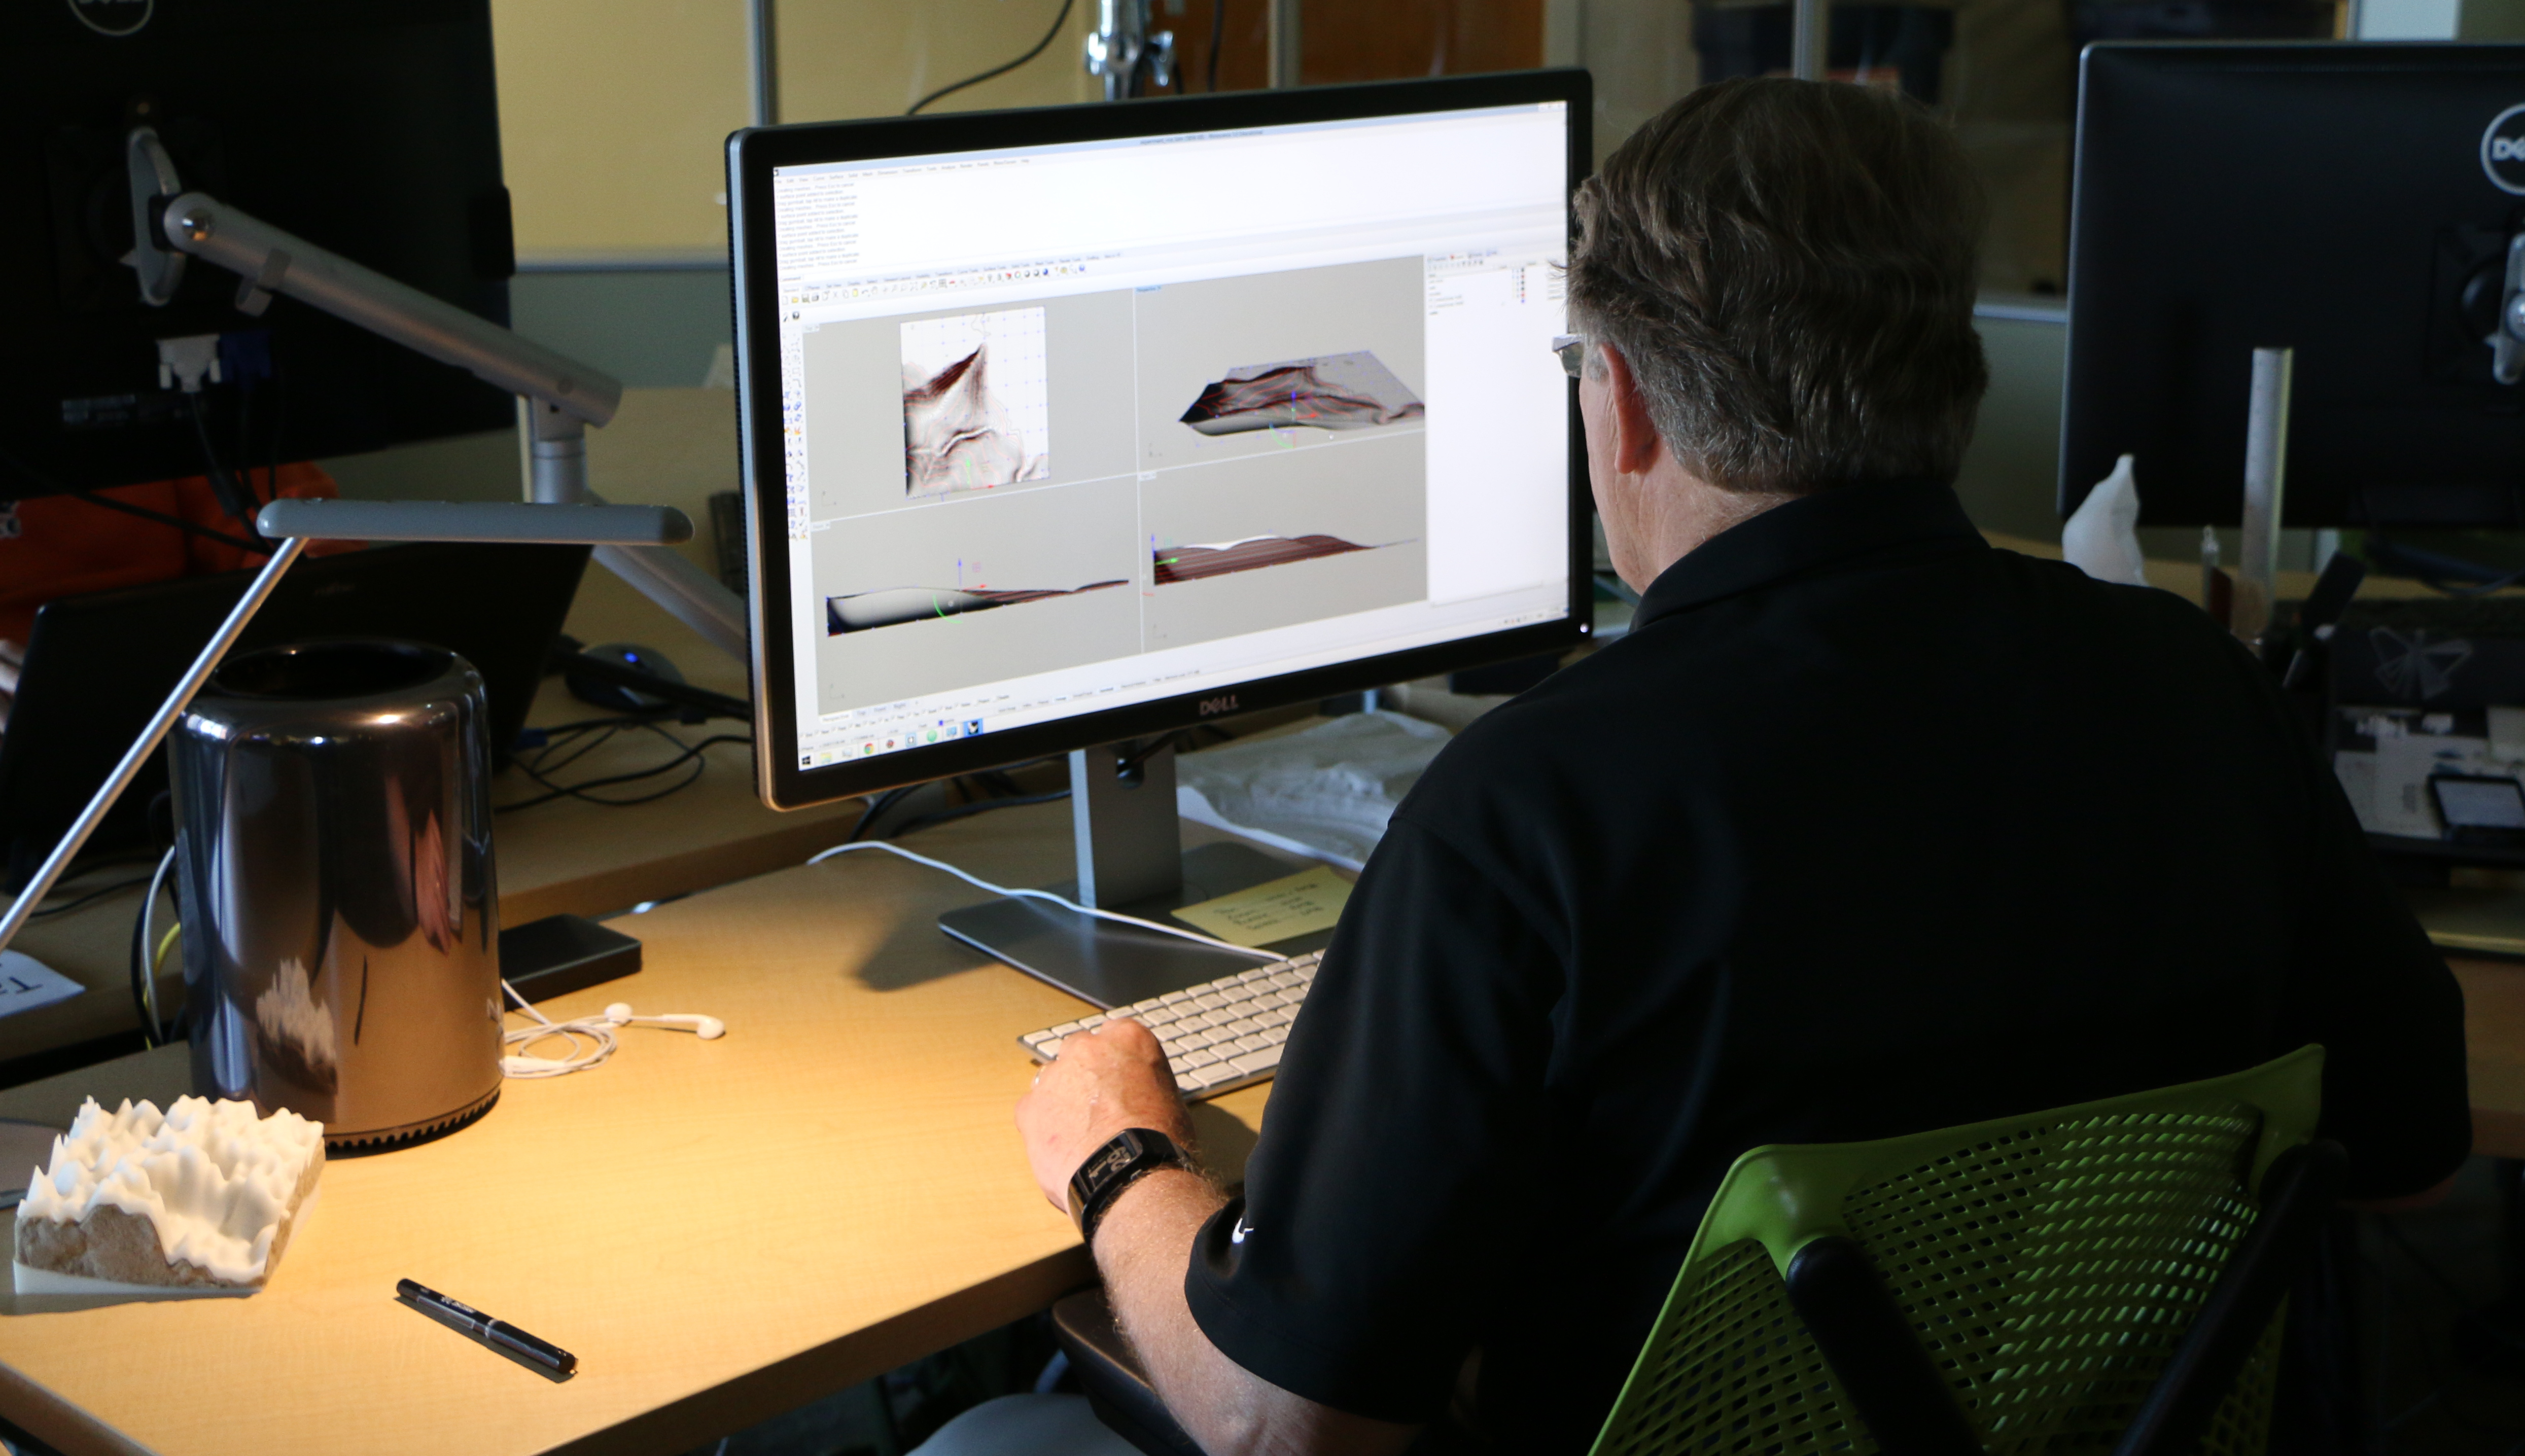
\includegraphics[width=0.48\textwidth]{images/experiments/art_rhino.jpg}
	\caption{Digital modeling -- 
	a participant digitally sculpts the study landscape in Rhinoceros
	using 3D contours as guides.}
	\label{fig:digital}
	%
	\vspace*{0.5em}
	%
	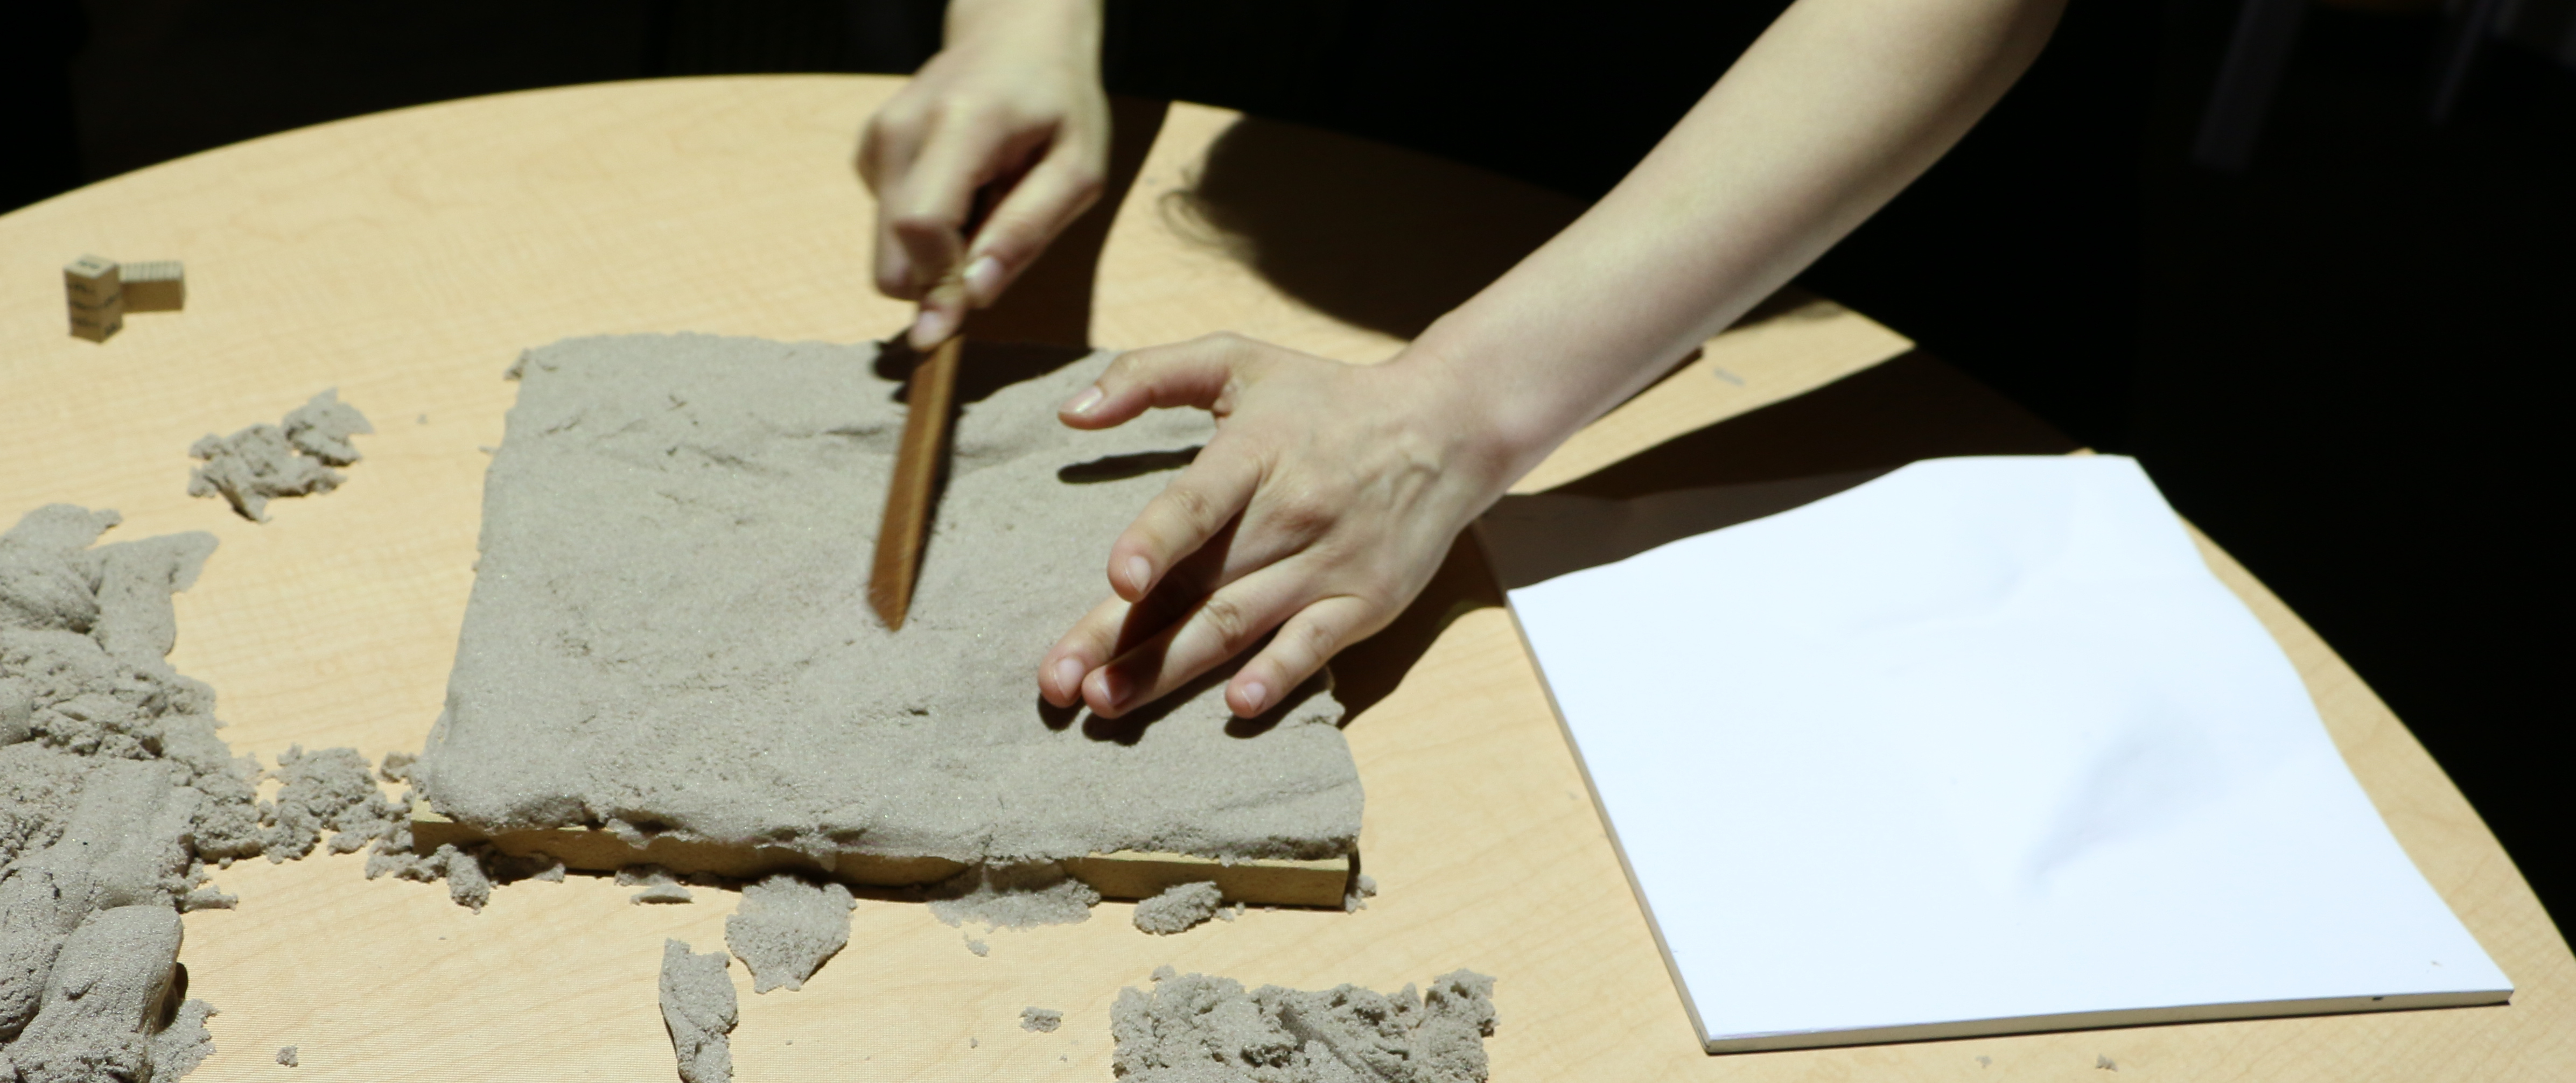
\includegraphics[width=0.48\textwidth]{images/experiments/connie_analog_1.jpg}
	\caption{Analog modeling -- 
	a participant sculpts the study landscape by hand
	using a physical model as a reference.}
	\label{fig:analog}
	%
	\vspace*{0.5em}
	%
	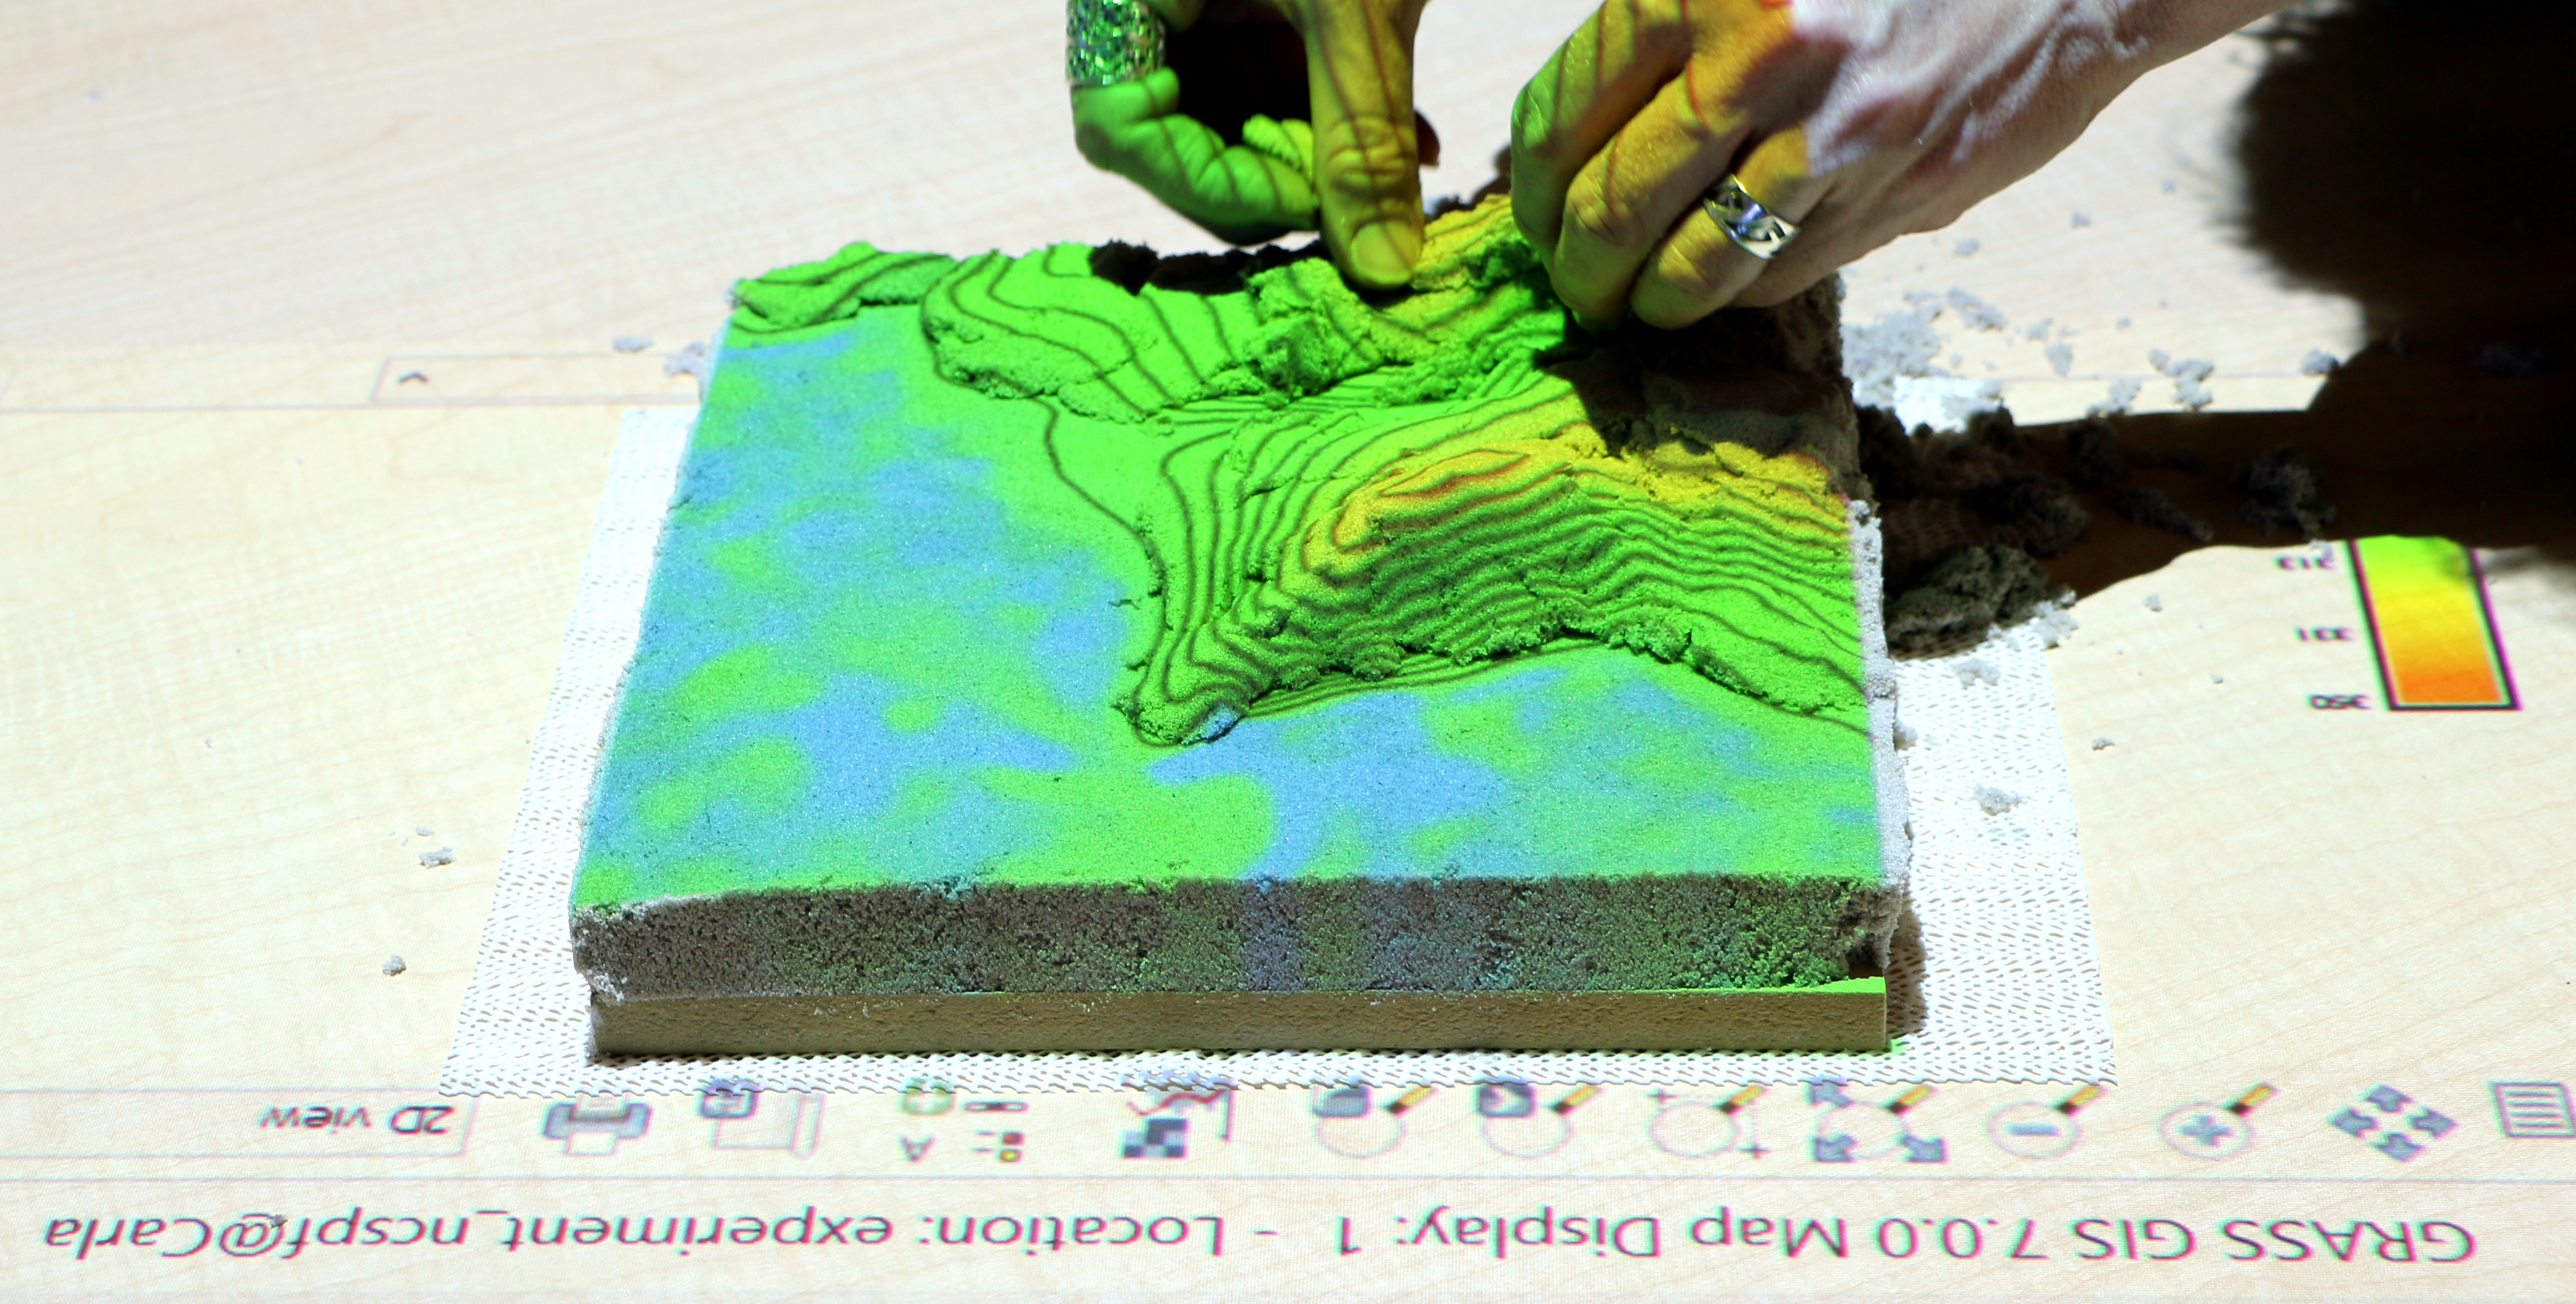
\includegraphics[width=0.48\textwidth]{images/experiments/carla_proj_aug.jpg}
	\caption{Tangible modeling --
	a participant sculpts the study landscape using
	the projected elevation and contour maps
	as guides.}
	\label{fig:tangible}
\end{center}
\label{fig:methods}
\end{figure}

% digital modeling
\paragraph{Digital modeling}
Participants had 10 minutes 
to digitally model the study landscape in Rhinoceros 5, 
a non-uniform rational basis spline 
(NURBS) based 3D modeling program
designed for precise freeform curve and surface modeling. \cite{Rhino}
After 10 minutes of training 
participants modeled the study landscape as a NURBS surface 
by vertically translating control points. 
They started with a flat NURBS surface that was 
divided into a 10 x 10 grid of control points.
As a reference their model space also included 
a locked representation of the study landscape as 3D contours. 
At any point participants could rebuild the surface 
with a higher density of control points for finer, more nuanced control. 
This method is relatively simple and 
analogous to basic actions in sculpture -- pushing and pulling. 
We developed and tested this method 
as a simple, straightforward technique for  
digital freeform surface modeling
that could be taught quickly, yet could produce an accurate model. 
Through testing we determined that 
novice users took approximately 10 minutes
to model the surface with a 10 x 10 grid of control points
before wanting to rebuild the surface with more control points.
% videos
See \url{https://youtu.be/dSyrHAuu698}
for a video demonstrating the training
and \url{https://youtu.be/vA1xwMSaGV4}
for a video demonstrating the digital 3D modeling task.

% choice of 3d modeling program
Different 3D modeling programs afford very different
interactions, modeling tools, data structures, and modes of representations. 
Developing a simple, intuitive modeling technique 
drove the choice of software in this study. 
After testing 3D modeling workflows in 
Rhinoceros, Vue, Maya, and SketchUp
we chose Rhinoceros 5 for this task because it 
is popular with designers such as architects, 
has a wide variety of modeling tools,
can precisely represent continuous surfaces, 
and has plugins for importing and exporting geographic data. 
To make a fair comparison 
between digital, analog, and tangible modeling,
the digital modeling technique 
needed to be relatively analogous to hand sculpting
-- i.e.~pushing and pulling rather than 
digitally painting in 3D, drafting in 3D, or stacking voxels.

% analog modeling
\paragraph{Analog modeling}
After a brief explanation and demonstration
participants had 10 minutes to sculpt 
the study landscape in polymer-enriched sand 
by hand or with a wooden sculpting tool.
They were given a CNC-routed model of the study landscape 
as a reference, a sculpting tool, and a 3D scale. 
Participants were shown how the 3D scale could be used to 
measure the height of the model. 
A lamp on the table cast shadows across the model for hillshading.
% videos
See \url{https://youtu.be/STYHUHNaWdY}
for a video demonstrating the analog 3D modeling task.

% tangible modeling
\paragraph{Tangible modeling}
After a minute long explanation and demonstration
participants had 10 minutes to sculpt
a projection-augmented, polymer-enriched sand model
of the study landscape 
either by hand or with a wooden sculpting tool.
Tangible Landscape was used to project 
an elevation map of the study landscape
with contours and a legend
onto participants' sand models as guide for sculpting. 
Participants were also given CNC routed reference model and 
a 3D scale ruled in map units. 
After an explanation of the contour map, elevation color table, and legend,
participants were shown how the 3D scale could be used to 
measure the elevation of their scale models.
% videos
See \url{https://youtu.be/1uEvzMJWh_E}
for a video demonstrating the tangible modeling task.

% data collection and analysis
\paragraph{Data collection and analysis}
We used Tangible Landscape to scan the finished models 
built using analog and tangible modeling.
The scans were captured as point clouds, interpolated 
as digital elevation models 
using the regularized spline with tension method,
and stored as raster maps in a GRASS GIS database. 
The NURBS surfaces modeled in Rhinoceros 
were exported as raster elevation maps,
imported into GRASS GIS, randomly resampled, 
re-interpolated using the regularized spline with tension method, 
and stored as raster maps in a GRASS GIS database. 
The data from Rhinoceros 
was randomly resampled and re-interpolated to account for 
differences and irregularities in resolution, data density, and point spacing.
For each set of models -- digital, analog, and tangible --
we computed raster statistics (i.e.~per cell statistics), 
topographic and morphometric parameters, 
and simulated water flow.

% ---------------------------
\subsection{Results}
% overall results
Overall participants performed best with tangible modeling.
%
The 3D maps of raster statistics and geospatial analyses in
Table \ref{table:topography} 
show how participants performed with each technology.
%
When digitally modeling with Rhinoceros 
participants tended to 
create very approximate massings of the topography
with serious errors in the interior space and
with indistinct landforms
that only hinted at the morphology of the landscape.
%
When they sculpted by hand
their models tended to be descriptive -- 
differing substantially from the reference model, but
accurately representing most of the landforms. 
%
Their performance improved 
with tangible modeling --
the resulting models
fit the reference better, 
had more defined topography, 
and accurately represented landforms.

% group results
We used pairwise comparison to study 
how performance varied between 
novices and experts (Fig. \ref{fig:comparison}).
After analyzing all participants' performance
we compared students with academics and professionals. 
Then we compared landscape architecture students with GIS students.
Finally we compared academics and professionals 
with and without 3D modeling expertise.
%
When participants are analyzed as groups 
-- as GIS students, landscape architecture students, 
academics and professionals without 3D modeling expertise, 
and academics and professionals with 3D modeling expertise -- 
these trends generally still hold, 
albeit with some very important exceptions.
%
Unlike all other groups, 
the 3D modeling experts performed well 
in the digital modeling task
with a very low standard deviation of difference, 
although they only hinted at the landforms. 
They, however, performed even better with tangible modeling,
accurately representing all of the landforms. 
%
These results show 
tangible modeling is intuitive 
and should be -- even for experts -- 
a better, faster tool 
for quick modeling tasks such as rapid ideation.

%\begin{figure*}[t]
%%\begin{center}
%\resizebox {\textwidth} {!} {\begin{tikzpicture}[grow = right,
	level 1/.style={sibling distance=12 em},
	level 2/.style={sibling distance=6 em},
	level distance = 14em,
	every node/.style = {shape=rectangle, 
		rounded corners,
		draw, 
		font=\footnotesize\sffamily,
		align=center,
		top color=white,
		bottom color=white}]
\node {Participants \\ 
	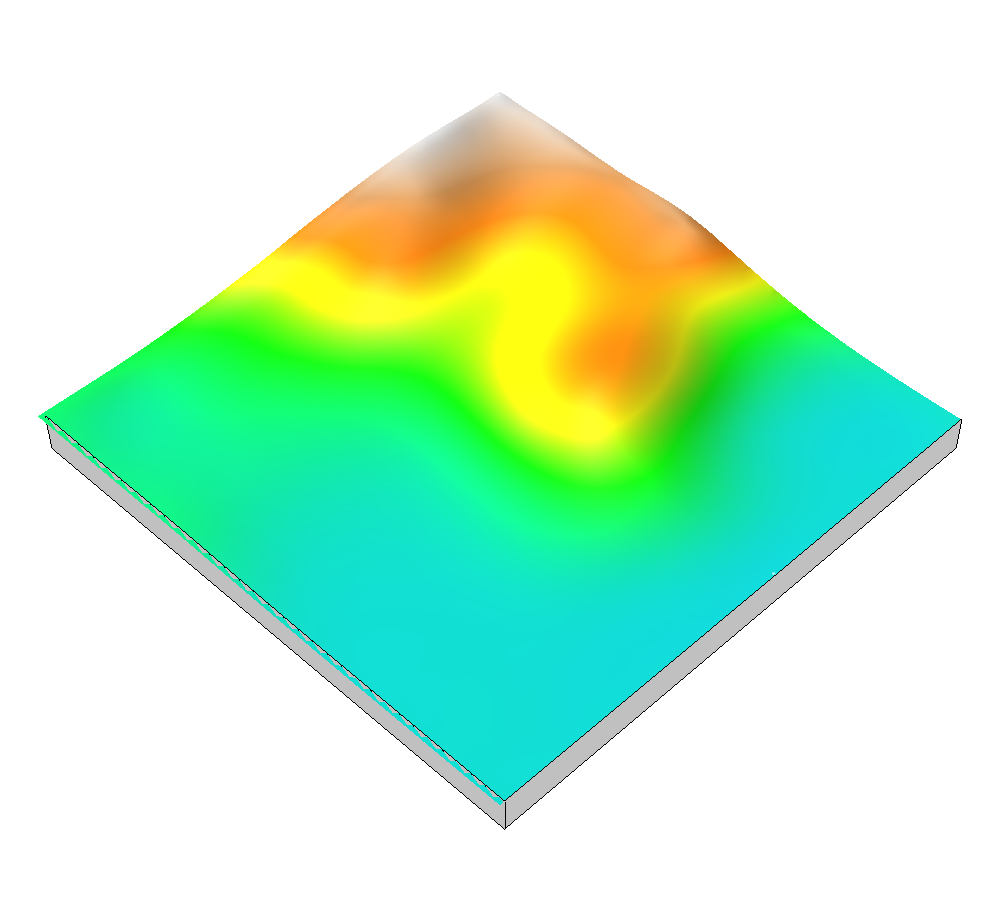
\includegraphics[width=0.08\textwidth]{images/render_3d/participants/mean_dem_1.png}
	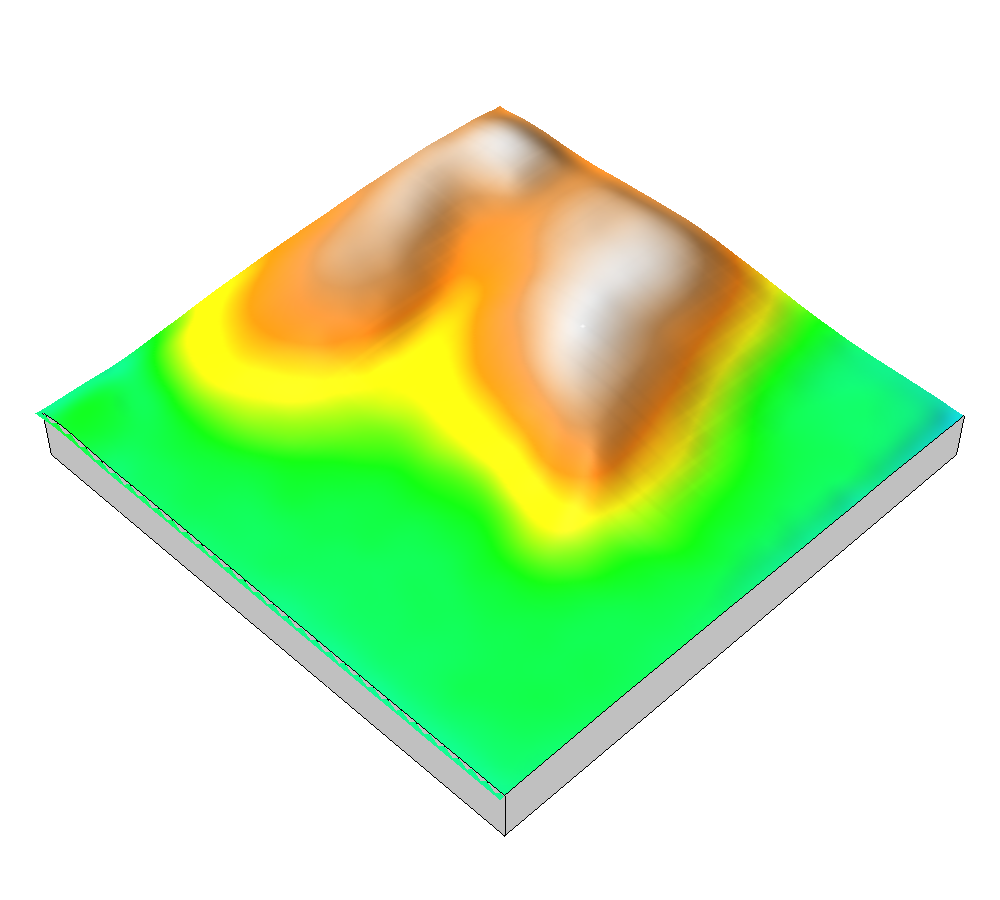
\includegraphics[width=0.08\textwidth]{images/render_3d/participants/mean_dem_2.png}
	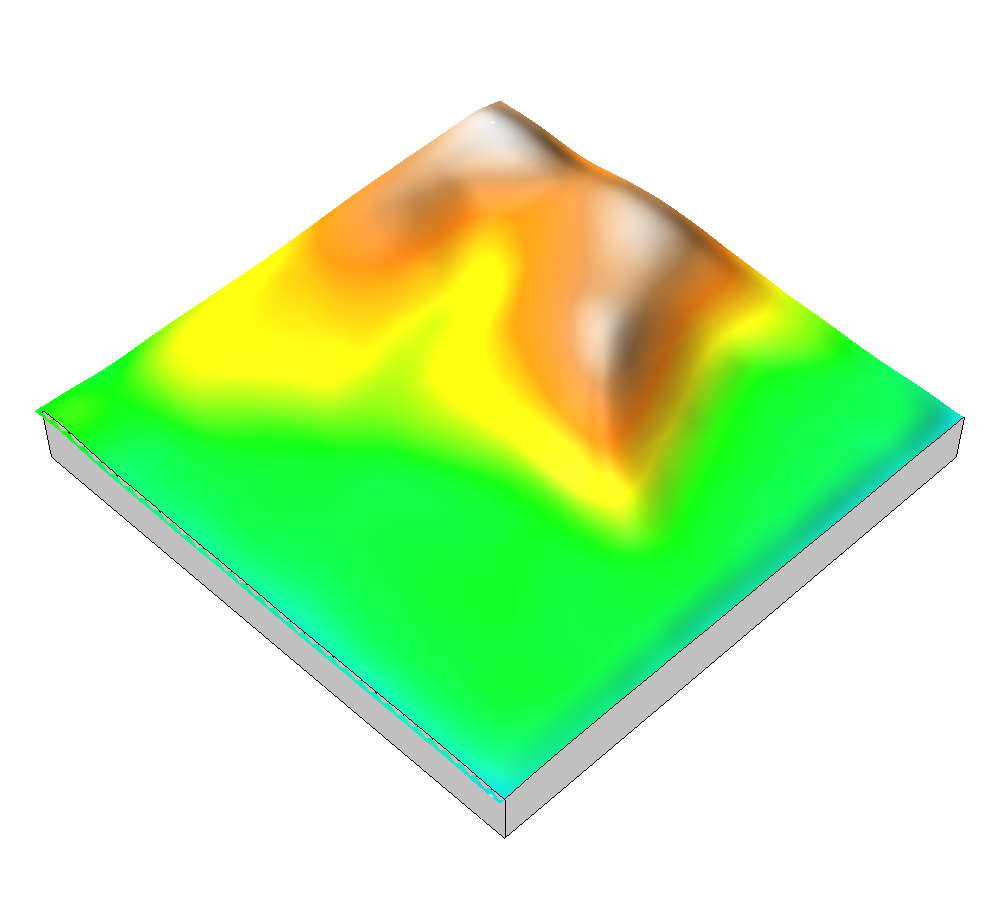
\includegraphics[width=0.08\textwidth]{images/render_3d/participants/mean_dem_3.png} \\
	\makebox[0.08\textwidth][c]{\scriptsize Digital}
	\makebox[0.08\textwidth][c]{\scriptsize Analog}
	\makebox[0.08\textwidth][c]{\scriptsize Tangible}
	}
	child { node {Students \\ 
		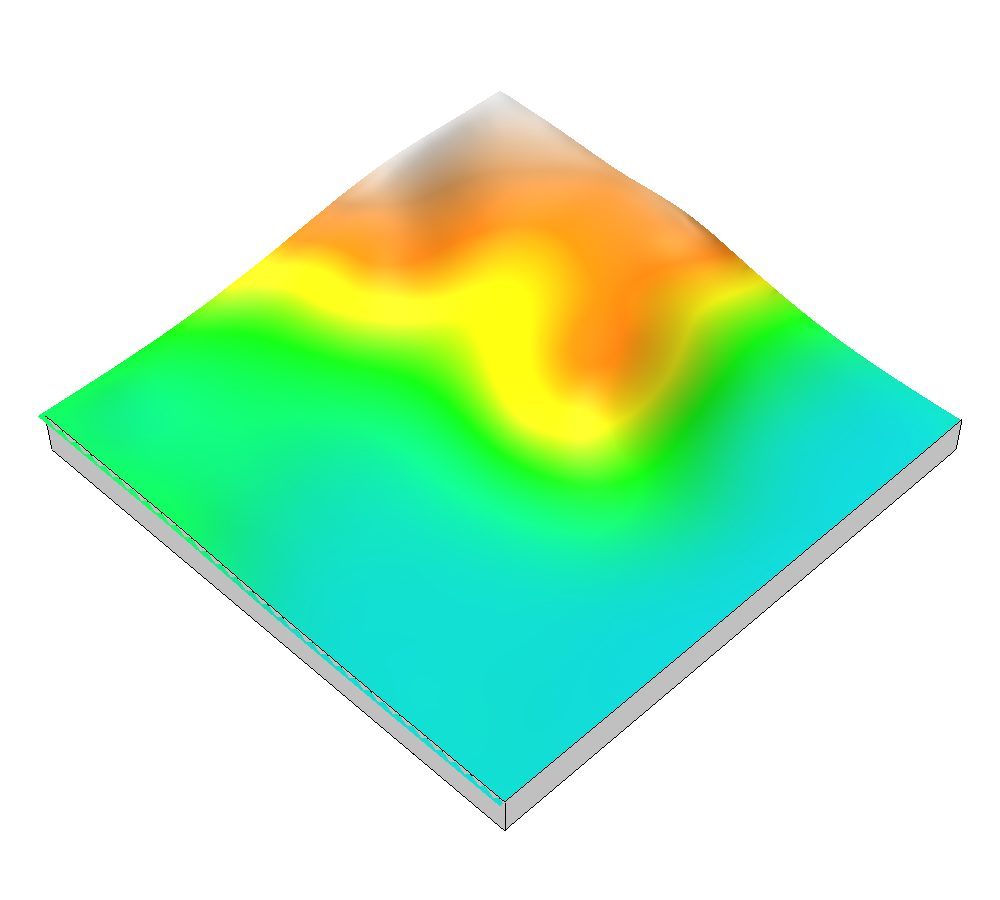
\includegraphics[width=0.08\textwidth]{images/render_3d/students/mean_dem_1.png}
		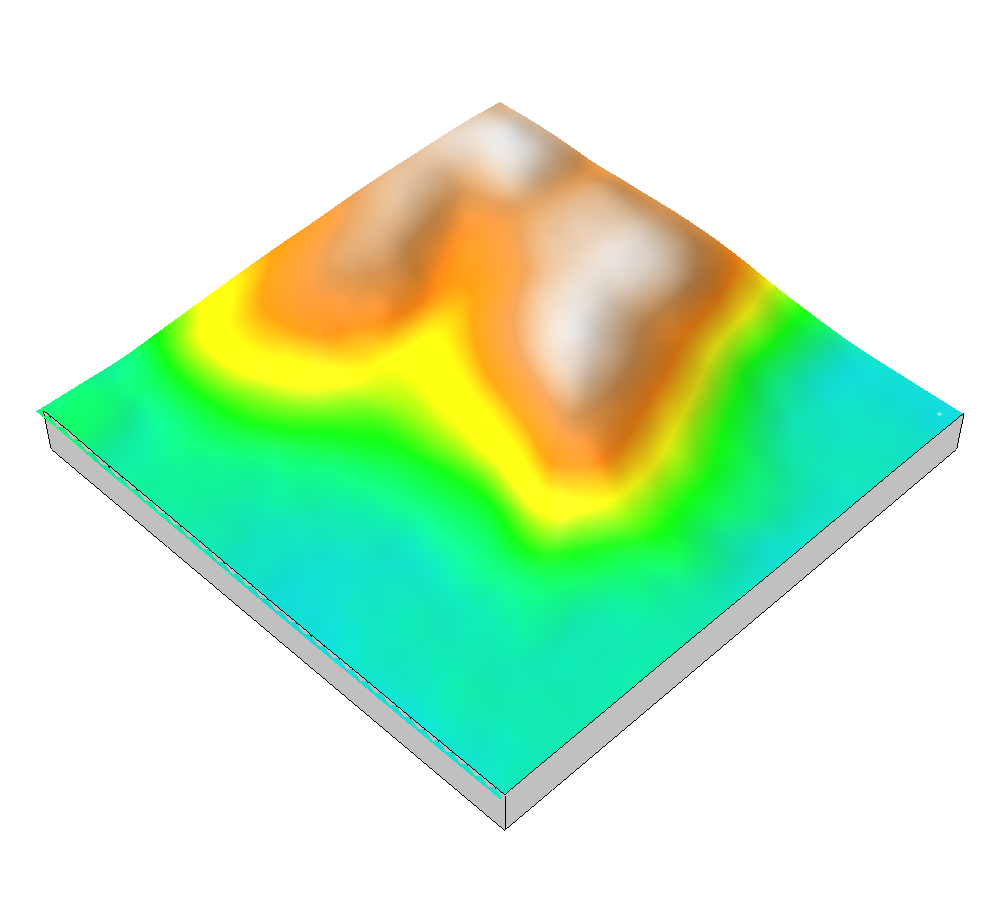
\includegraphics[width=0.08\textwidth]{images/render_3d/students/mean_dem_2.png}
		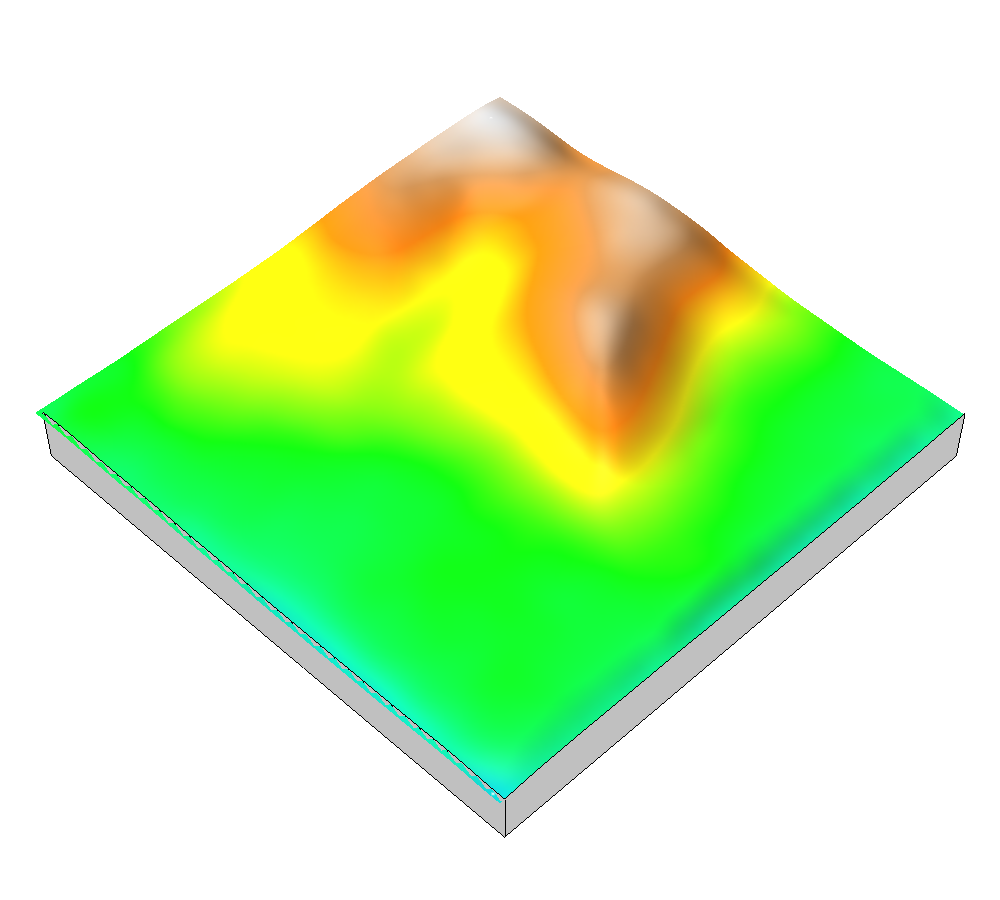
\includegraphics[width=0.08\textwidth]{images/render_3d/students/mean_dem_3.png}
		}
		child { node {Landscape architecture \\ 
			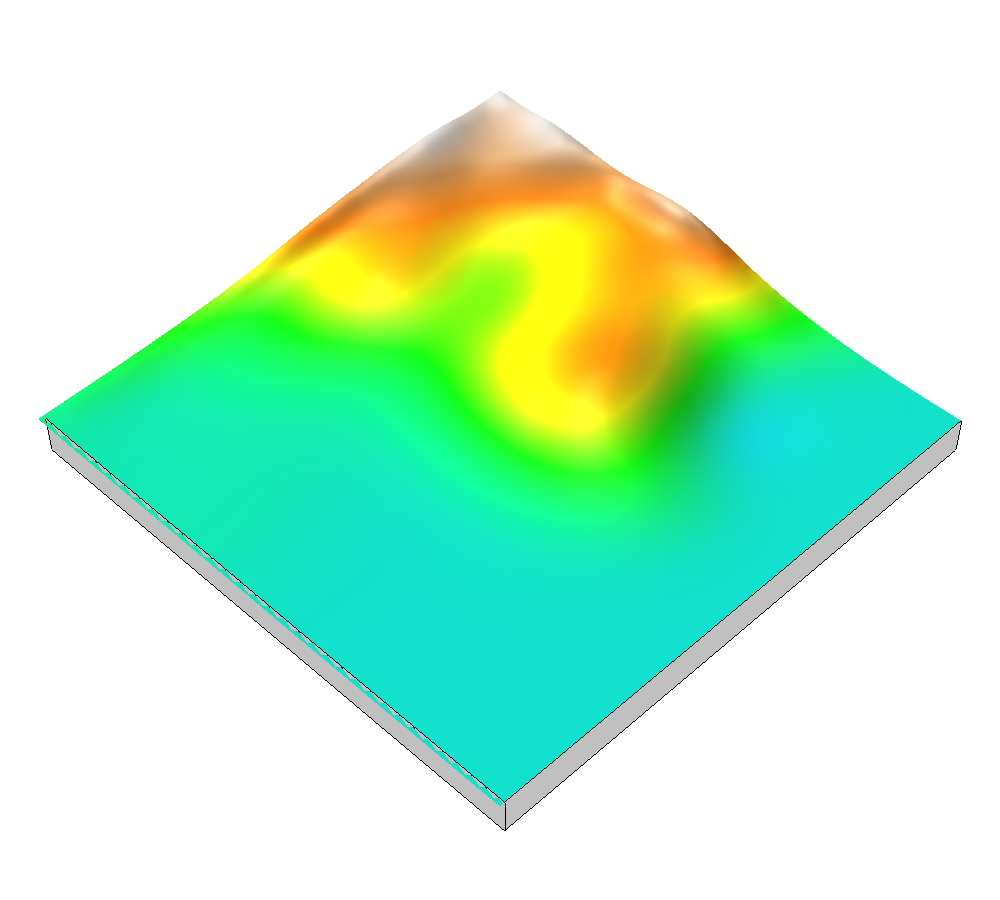
\includegraphics[width=0.08\textwidth]{images/render_3d/landscape_students/mean_dem_1.png}
			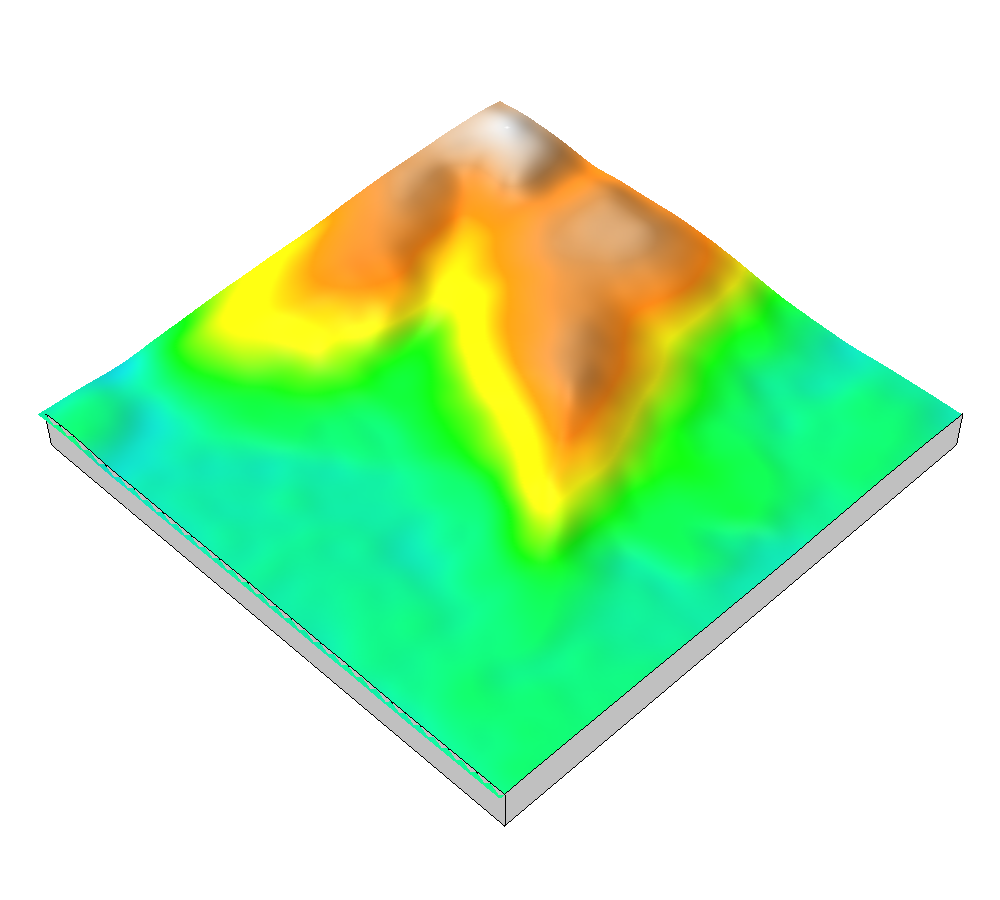
\includegraphics[width=0.08\textwidth]{images/render_3d/landscape_students/mean_dem_2.png}
			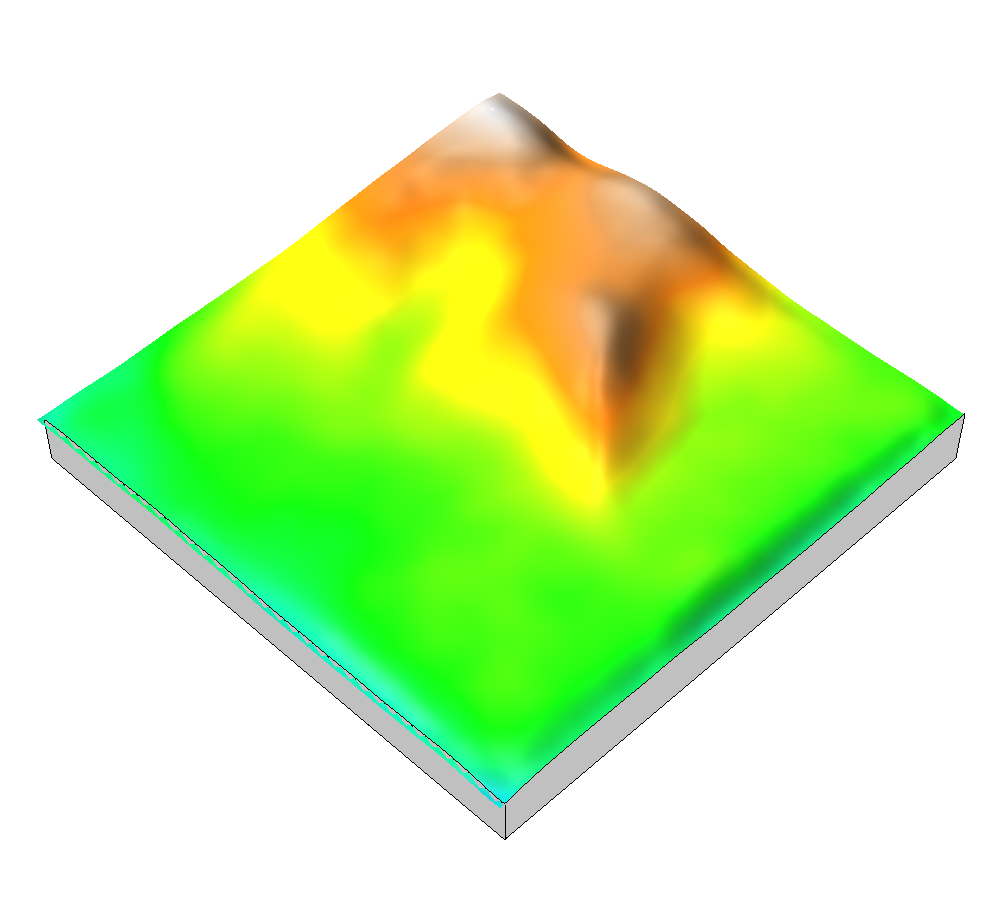
\includegraphics[width=0.08\textwidth]{images/render_3d/landscape_students/mean_dem_3.png}
			}
			}
		child { node {GIS \\ 
			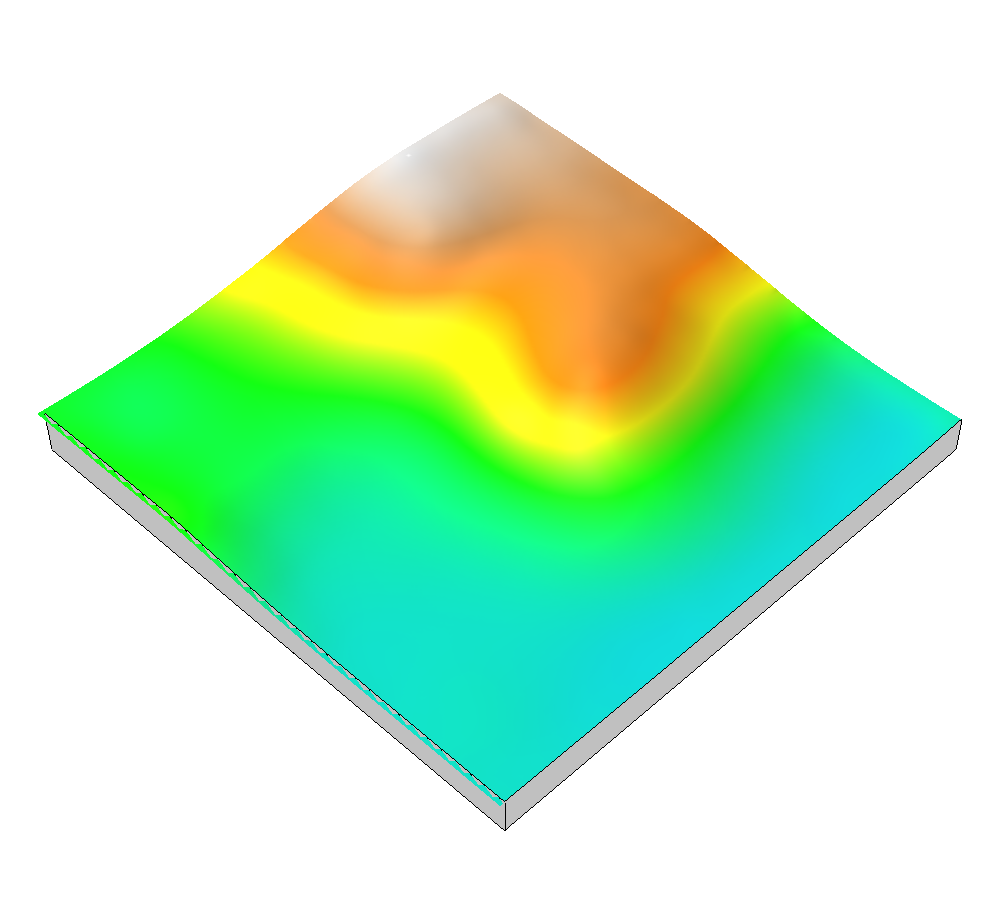
\includegraphics[width=0.08\textwidth]{images/render_3d/gis_students/mean_dem_1.png}
			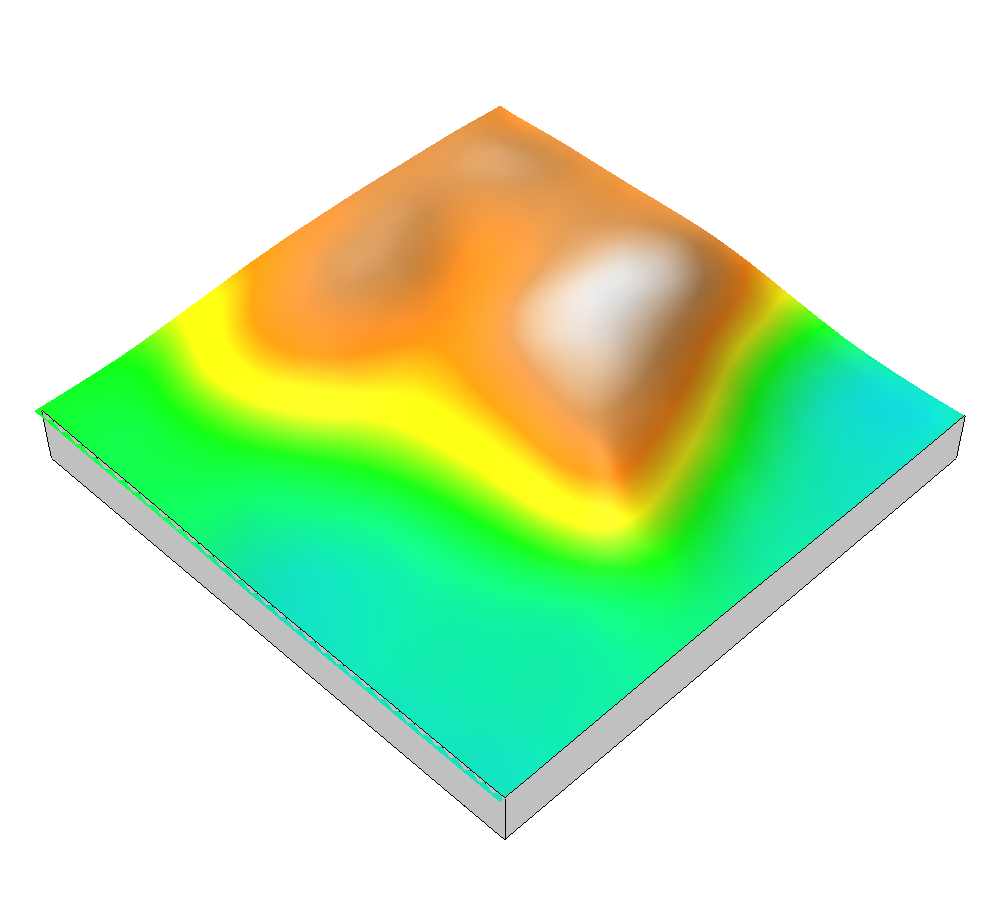
\includegraphics[width=0.08\textwidth]{images/render_3d/gis_students/mean_dem_2.png}
			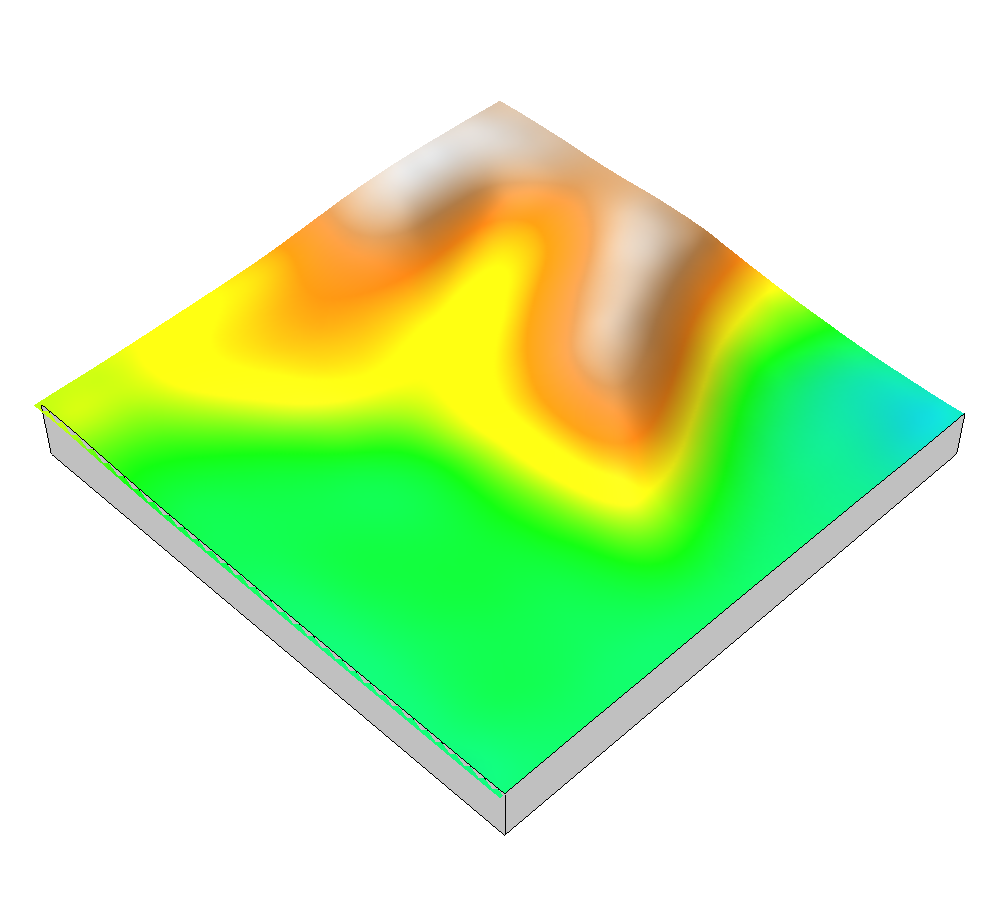
\includegraphics[width=0.08\textwidth]{images/render_3d/gis_students/mean_dem_3.png}
			}
			}
		}
	child { node {Professionals \\ 
		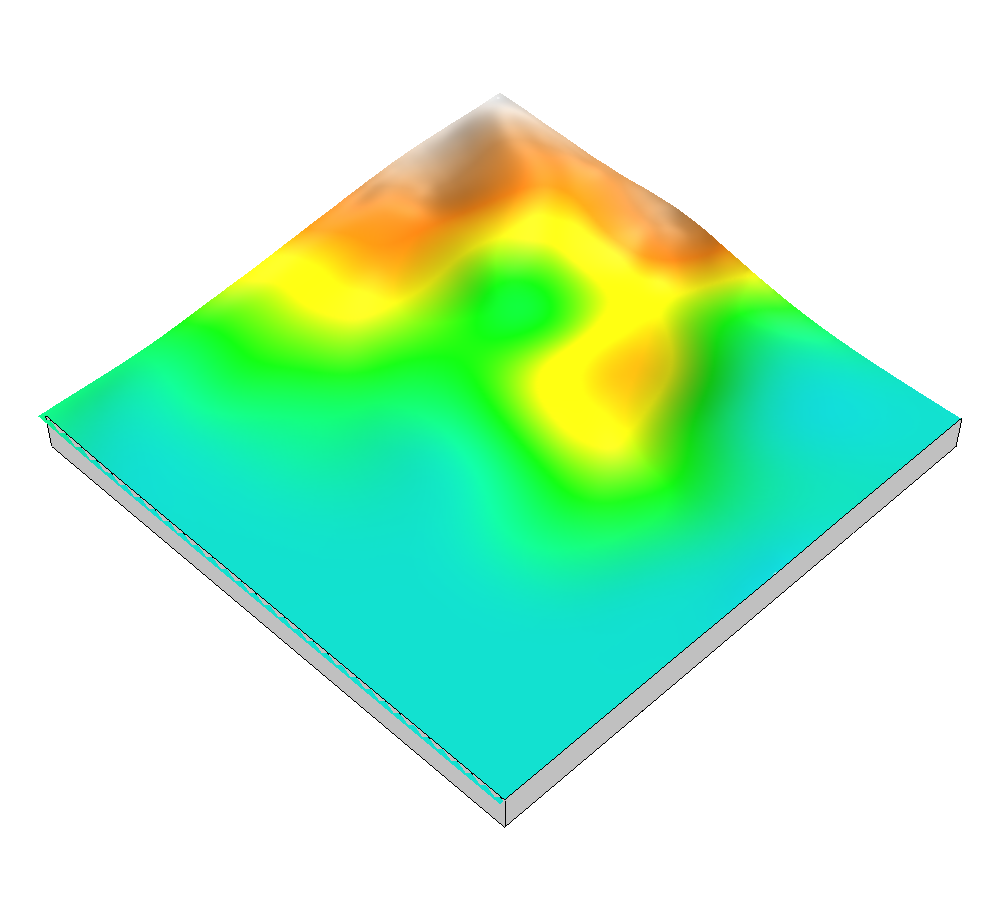
\includegraphics[width=0.08\textwidth]{images/render_3d/professionals/mean_dem_1.png}
		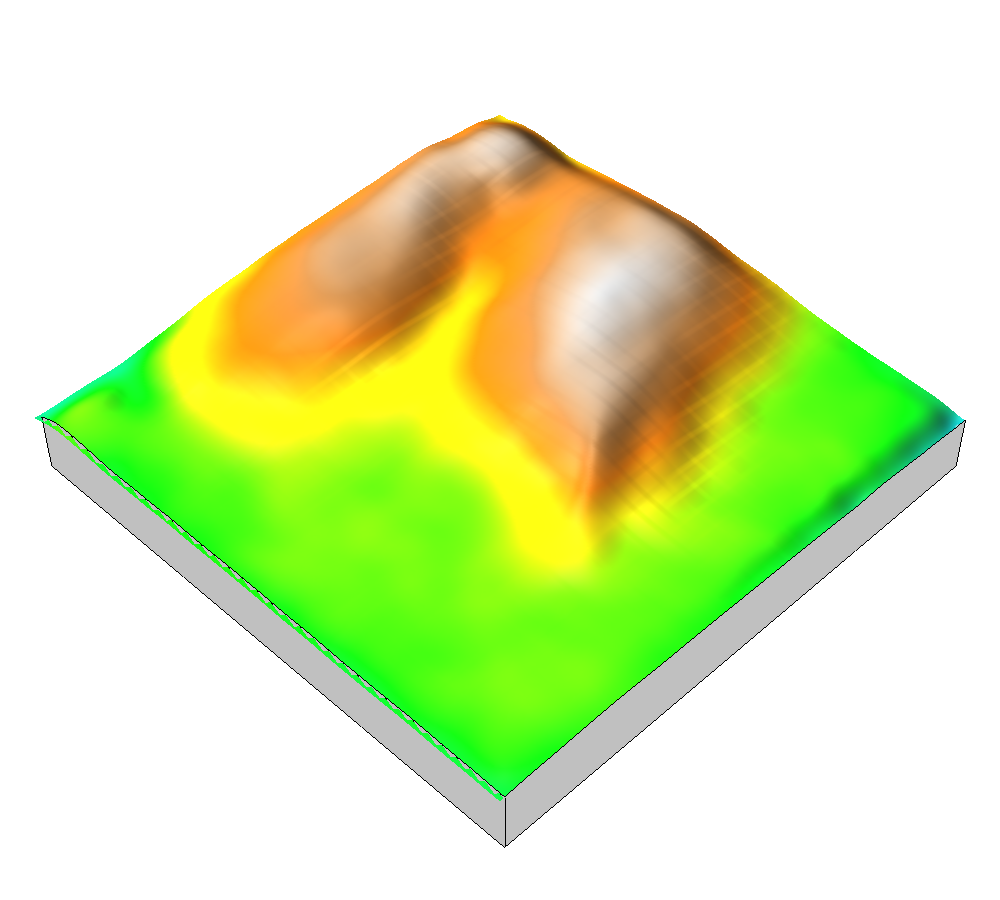
\includegraphics[width=0.08\textwidth]{images/render_3d/professionals/mean_dem_2.png}
		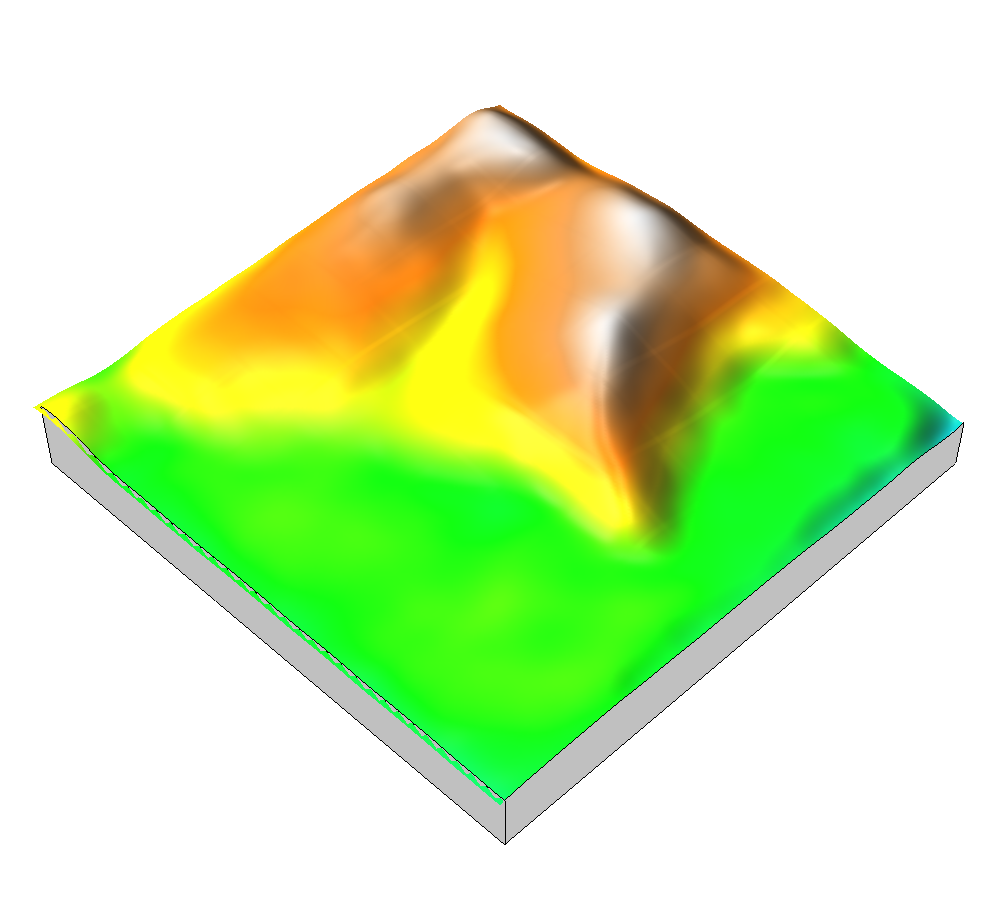
\includegraphics[width=0.08\textwidth]{images/render_3d/professionals/mean_dem_3.png}
		}
		child { node {3D novices \\ 
			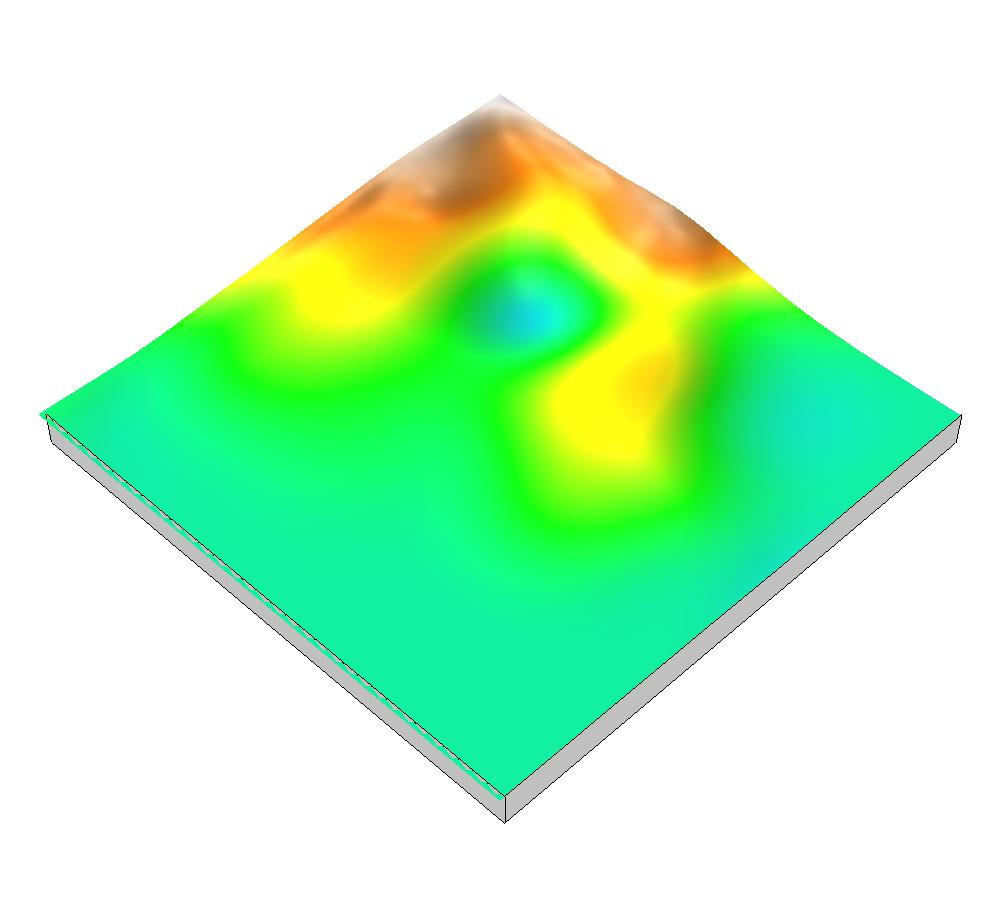
\includegraphics[width=0.08\textwidth]{images/render_3d/3d_novices/mean_dem_1.png}
			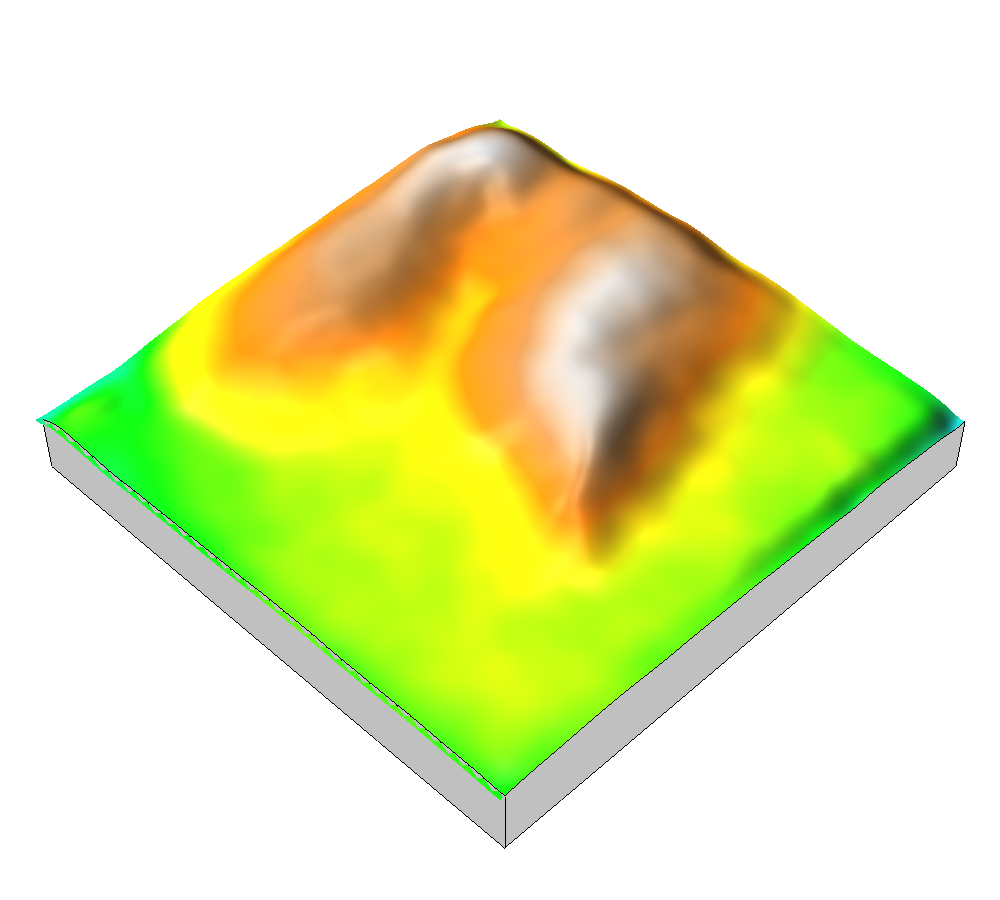
\includegraphics[width=0.08\textwidth]{images/render_3d/3d_novices/mean_dem_2.png}
			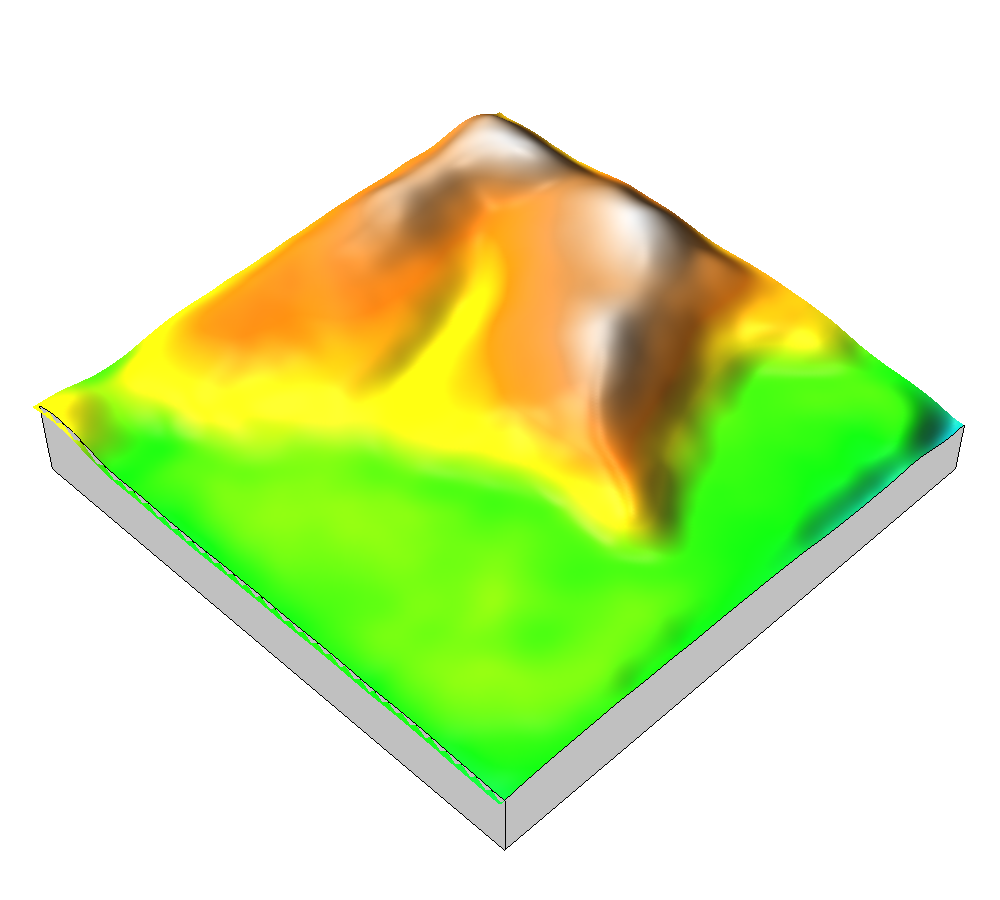
\includegraphics[width=0.08\textwidth]{images/render_3d/3d_novices/mean_dem_3.png}
			}
			}
		child { node {3D experts \\ 
			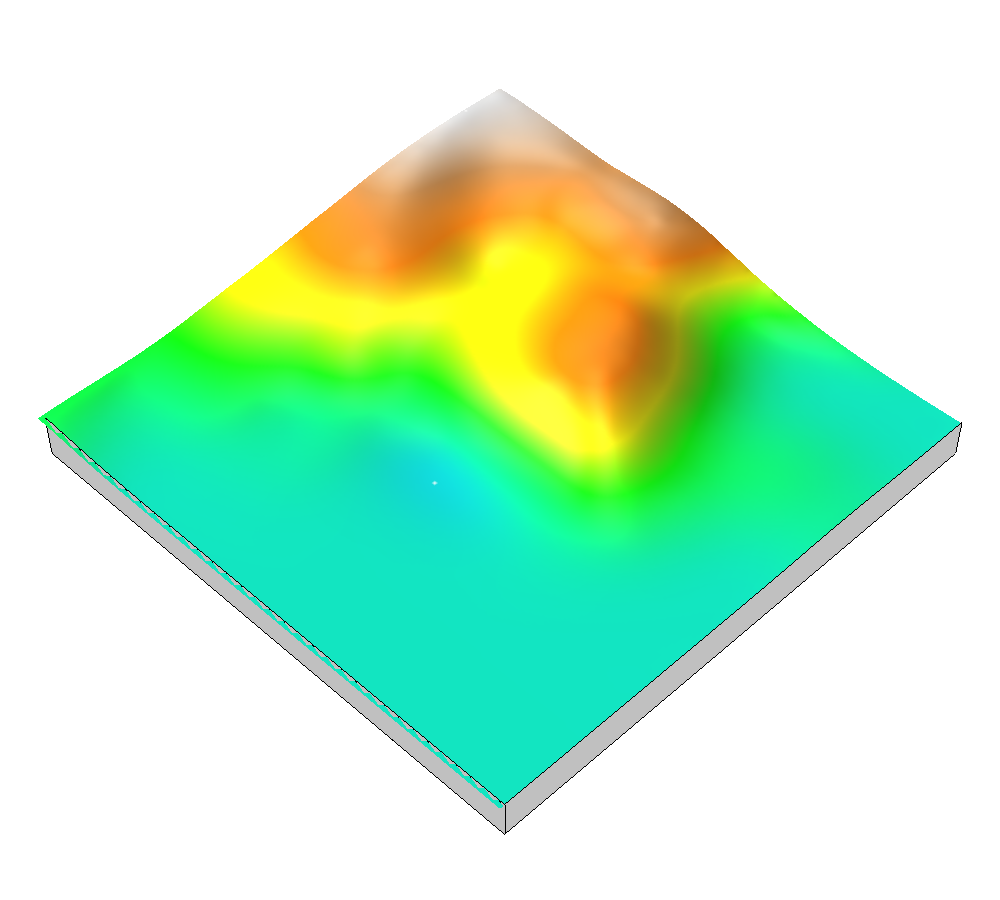
\includegraphics[width=0.08\textwidth]{images/render_3d/3d_experts/mean_dem_1.png}
			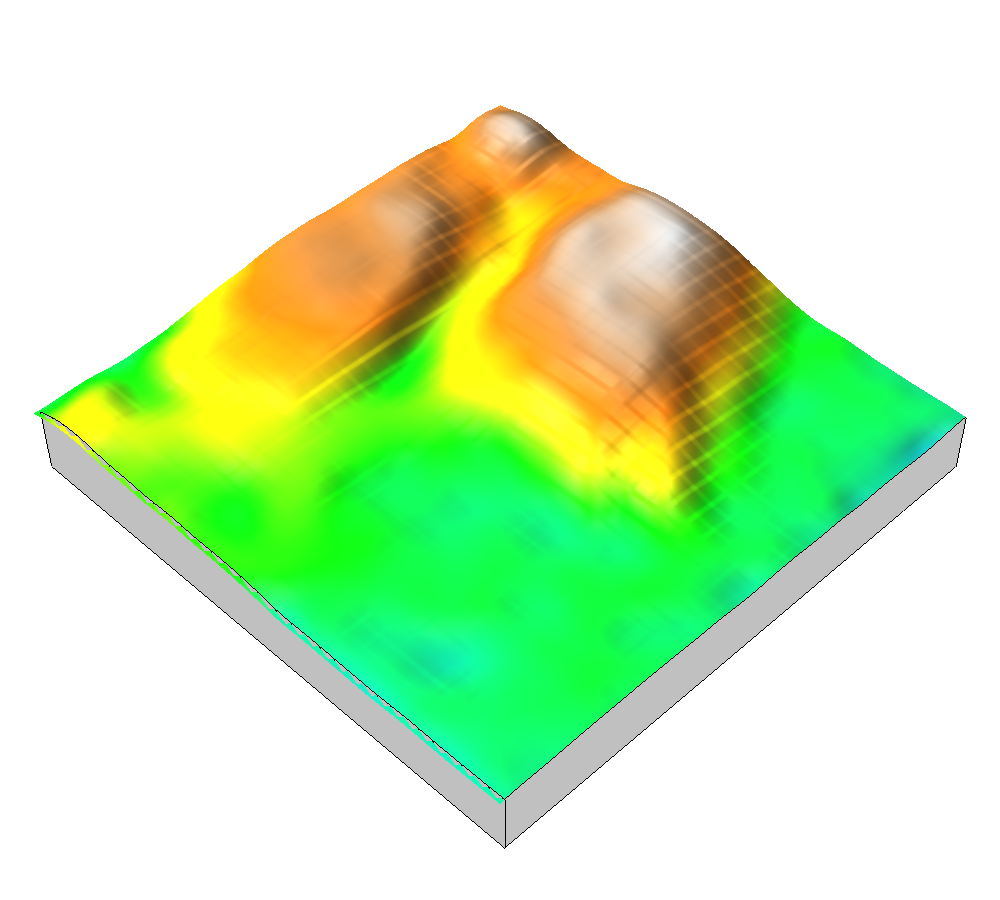
\includegraphics[width=0.08\textwidth]{images/render_3d/3d_experts/mean_dem_2.png}
			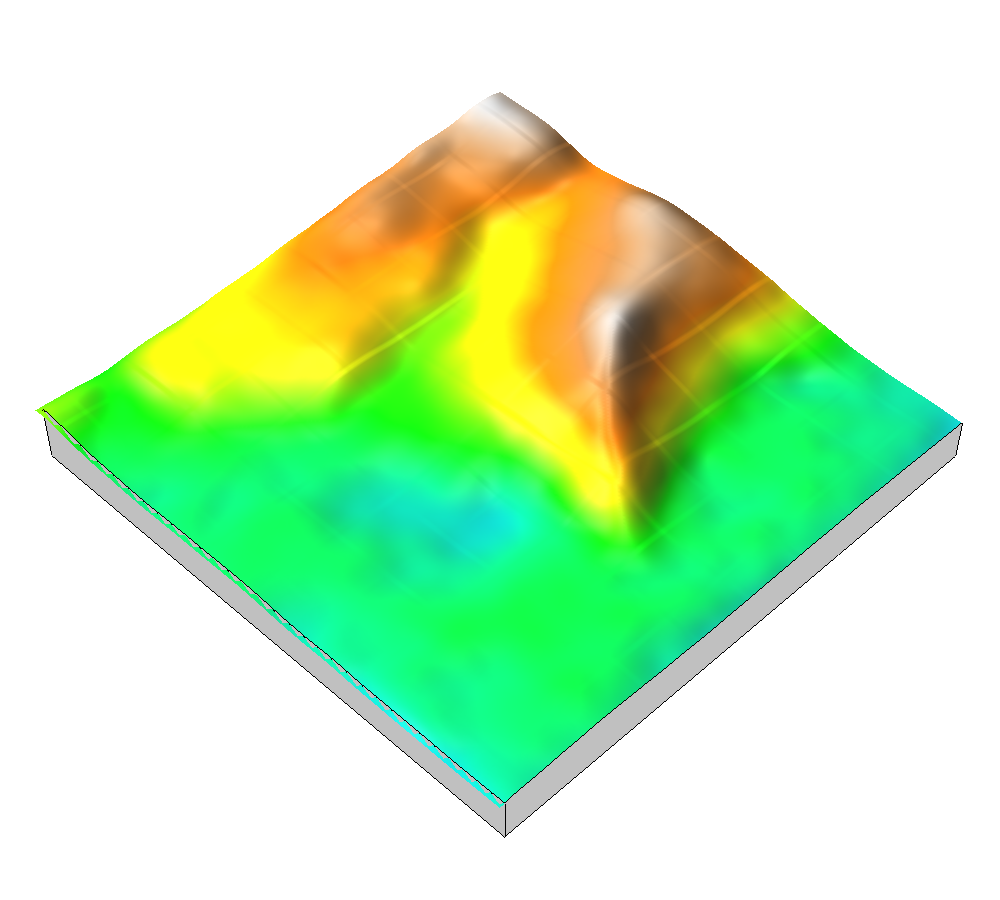
\includegraphics[width=0.08\textwidth]{images/render_3d/3d_experts/mean_dem_3.png}
			}
			}
};
\end{tikzpicture}
}
%\caption{Pairwise comparison of the mean digital elevation models 
%by category of participants.}
%\label{fig:comparison}
%%\end{center}
%\end{figure*}

%\begin{figure*}[t]
%\includestandalone[width=\textwidth]{comparison}
%\caption{Pairwise comparison of the mean digital elevation models 
%by category of participants.}
%\label{fig:comparison}
%\end{figure*}

\begin{figure*}[t]
\includegraphics[width=\textwidth]{tangible_topography-figure0.pdf}
\caption{Pairwise comparison of the mean digital elevation models 
by category of participants.}
\label{fig:comparison}
\end{figure*}

% ---------------------------- TOPOGRAPHY ---------------------------- 
\begin{table*}[h]
\small\sf\centering
\caption{Topographic experiment: maps of raster statistics and geospatial analyses draped over 3D topography for all participants.}
\ra{1.3}
\begin{tabular}{m{0.16\textwidth} m{0.18\textwidth} m{0.18\textwidth} m{0.18\textwidth} m{0.18\textwidth}}
\toprule
& \multicolumn{1}{c}{Reference} & \multicolumn{1}{c}{Digital} & \multicolumn{1}{c}{Analog}  & \multicolumn{1}{c}{Tangible}\\
\midrule
%
Mean elevation \par \vspace{0.5em} 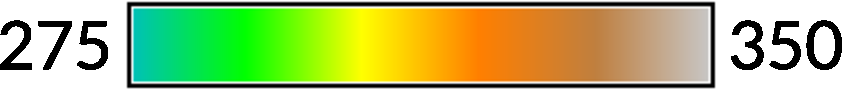
\includegraphics[width=0.16\textwidth]{images/legends/elevation_legend_1.pdf} & 
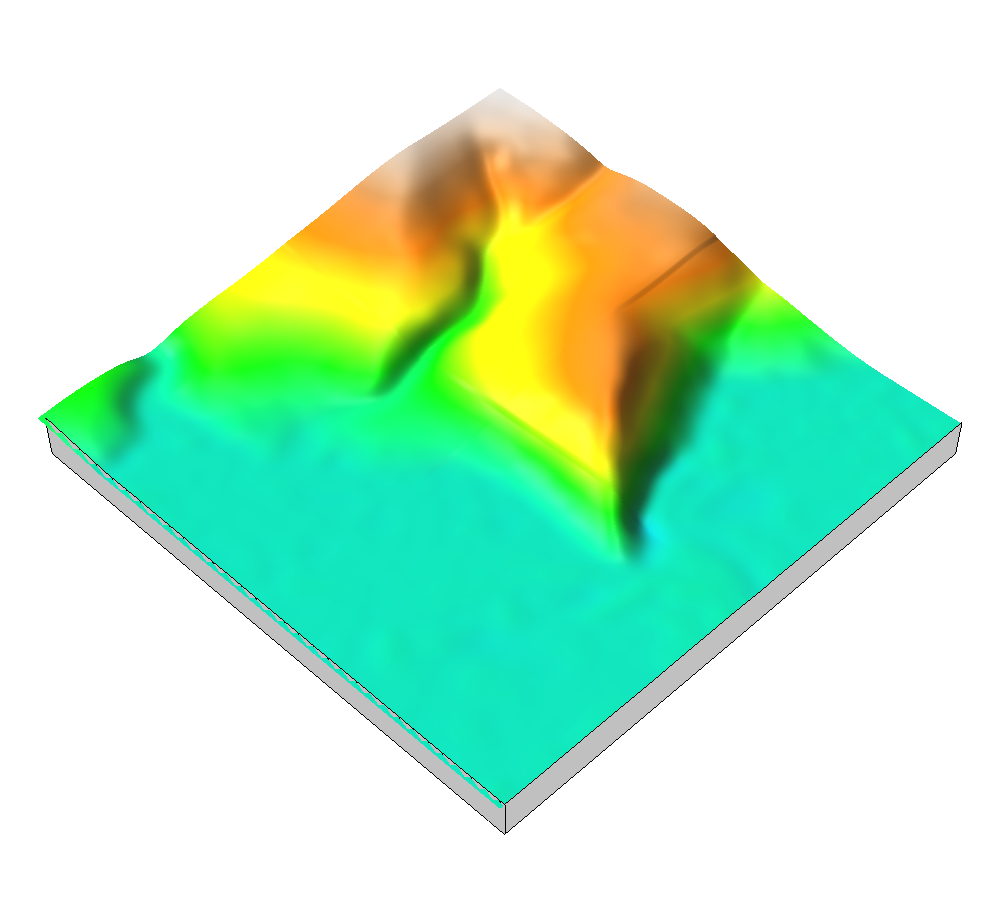
\includegraphics[width=0.18\textwidth]{images/render_3d/participants/dem_1.png} &
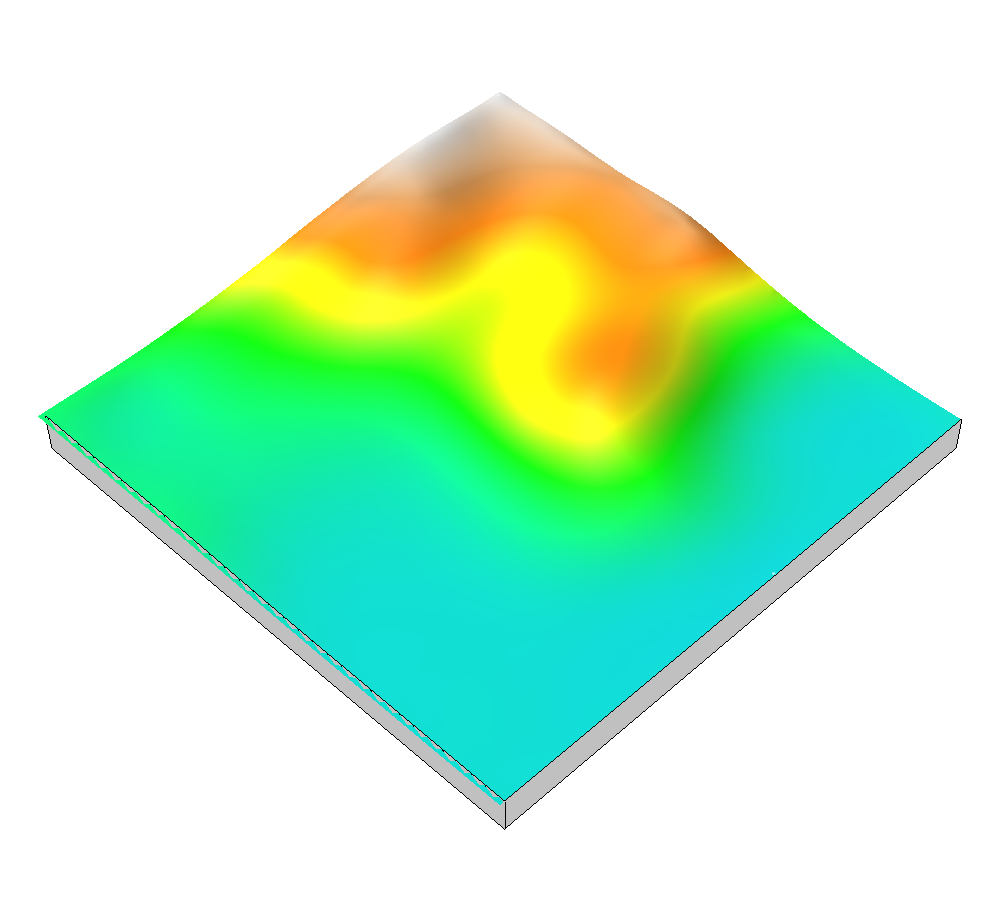
\includegraphics[width=0.18\textwidth]{images/render_3d/participants/mean_dem_1.png} &
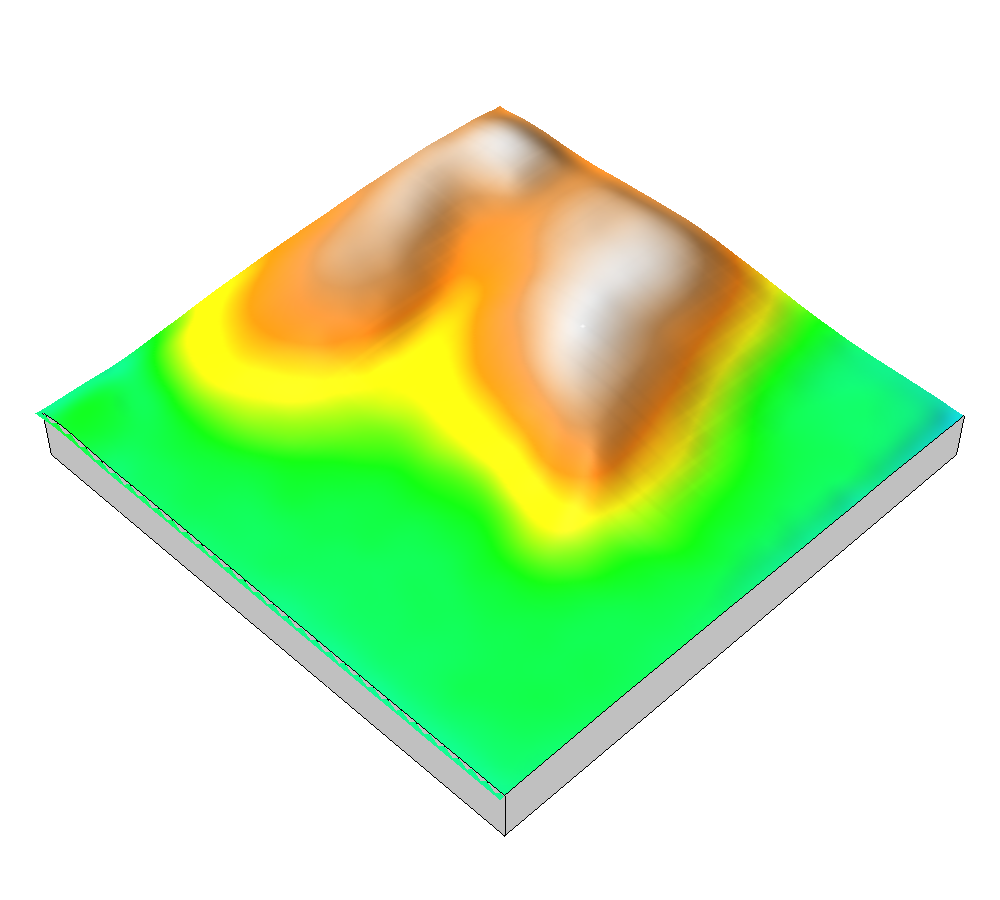
\includegraphics[width=0.18\textwidth]{images/render_3d/participants/mean_dem_2.png} &
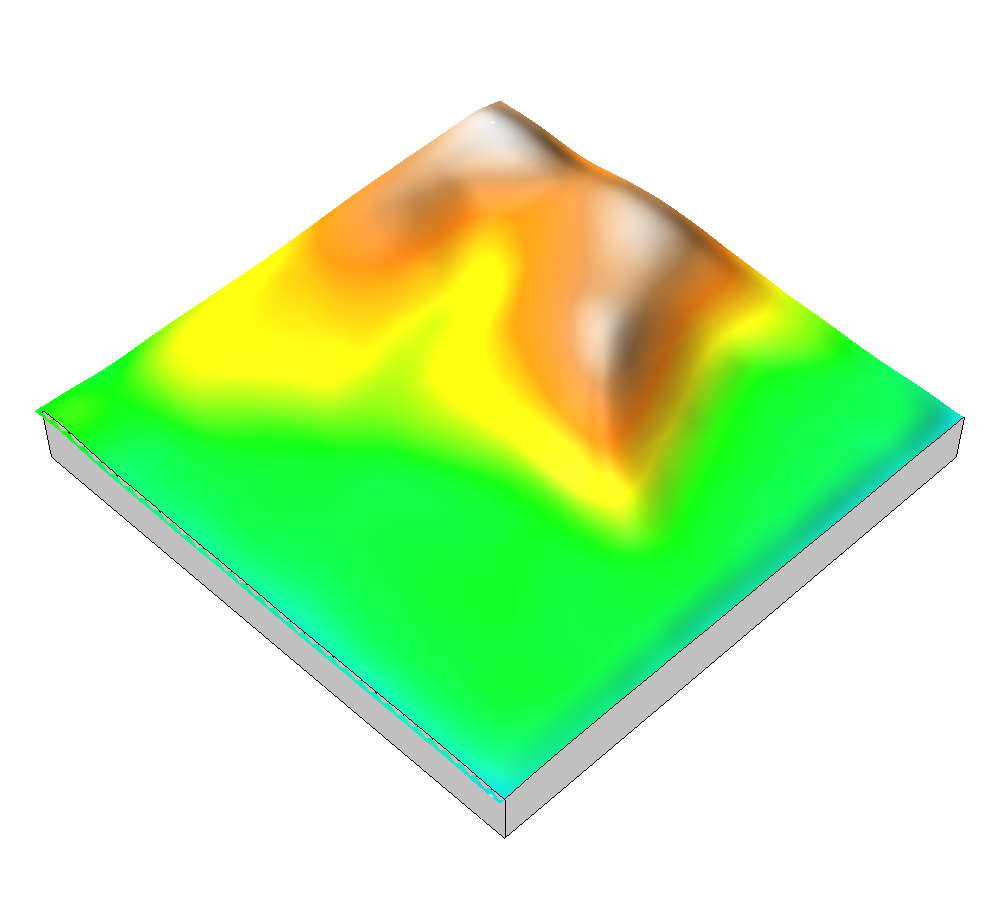
\includegraphics[width=0.18\textwidth]{images/render_3d/participants/mean_dem_3.png}\\
%
Stdev.~of elevations \par \vspace{0.5em} 
\includegraphics[width=0.16\textwidth]{images/legends/stdev_legend.pdf} & 
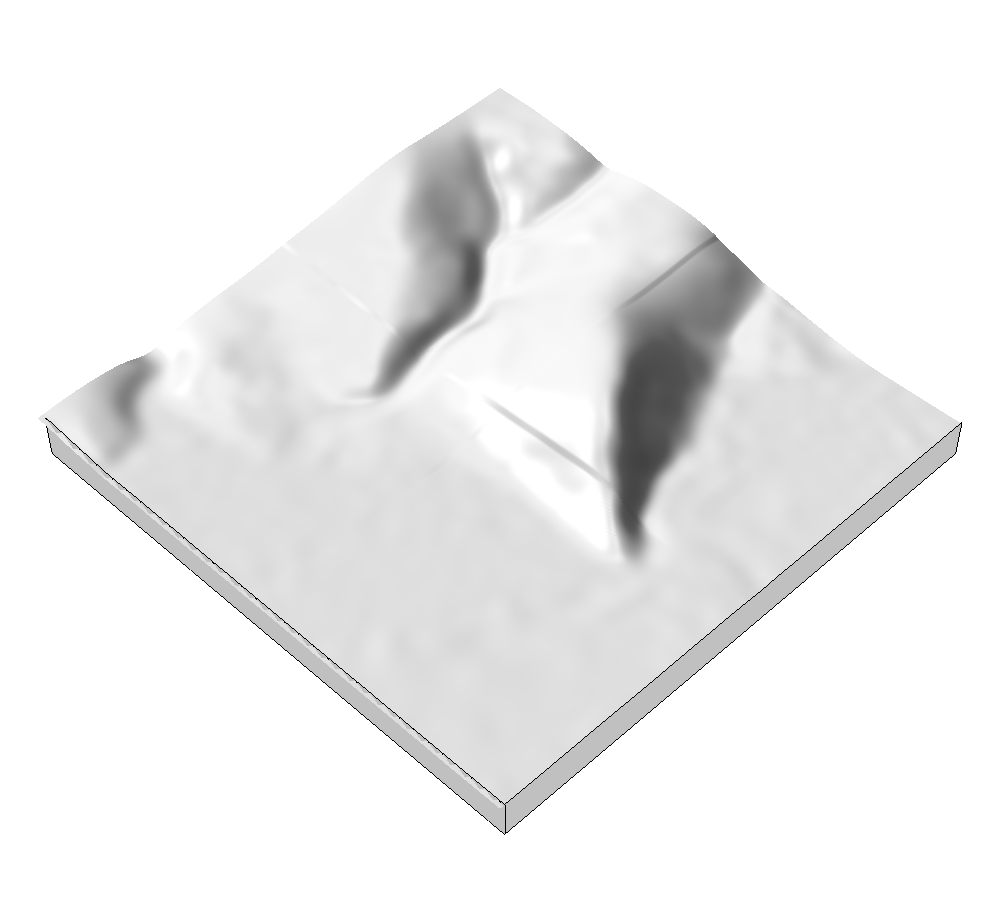
\includegraphics[width=0.18\textwidth]{images/render_3d/participants/dem_difference_1.png} &
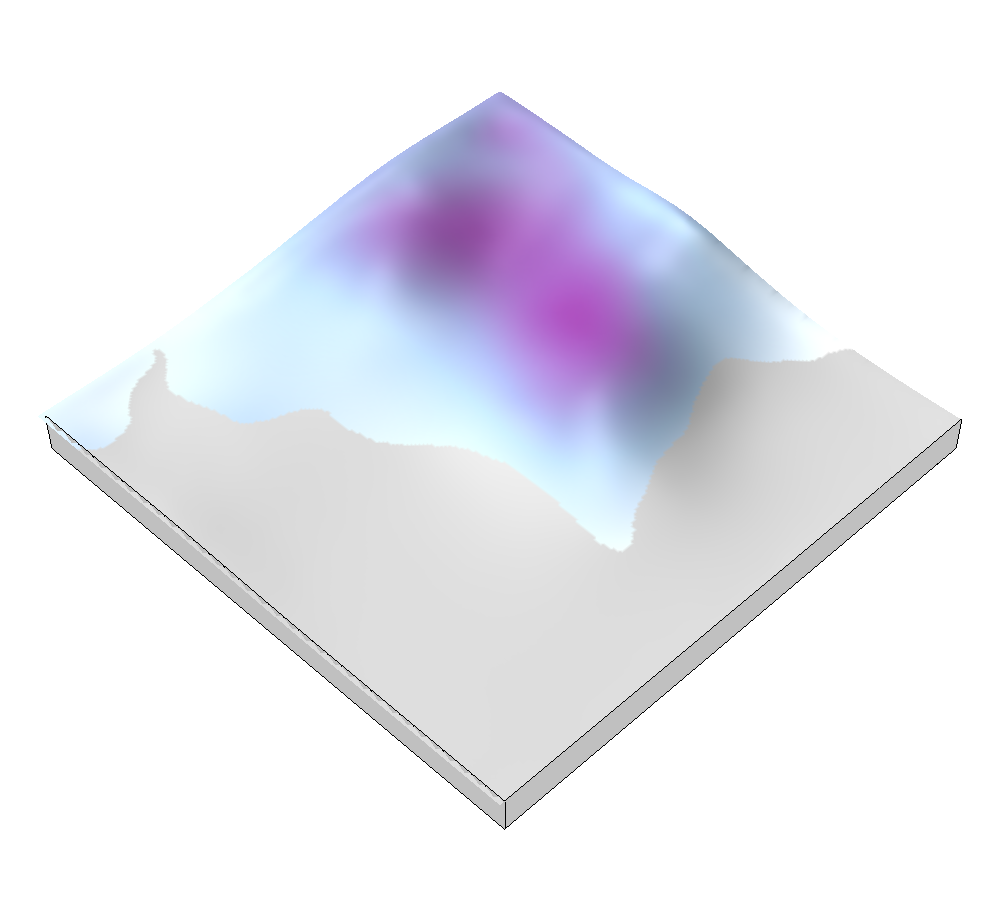
\includegraphics[width=0.18\textwidth]{images/render_3d/participants/stdev_dem_1.png} &
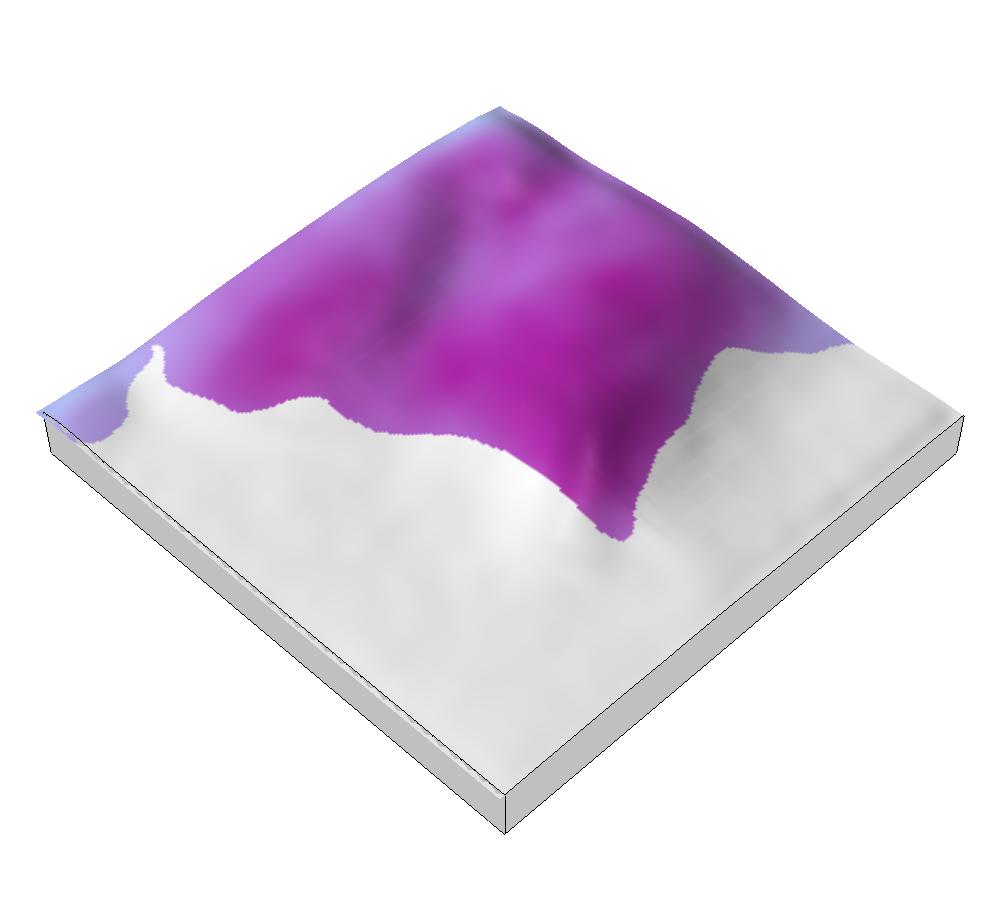
\includegraphics[width=0.18\textwidth]{images/render_3d/participants/stdev_dem_2.png} &
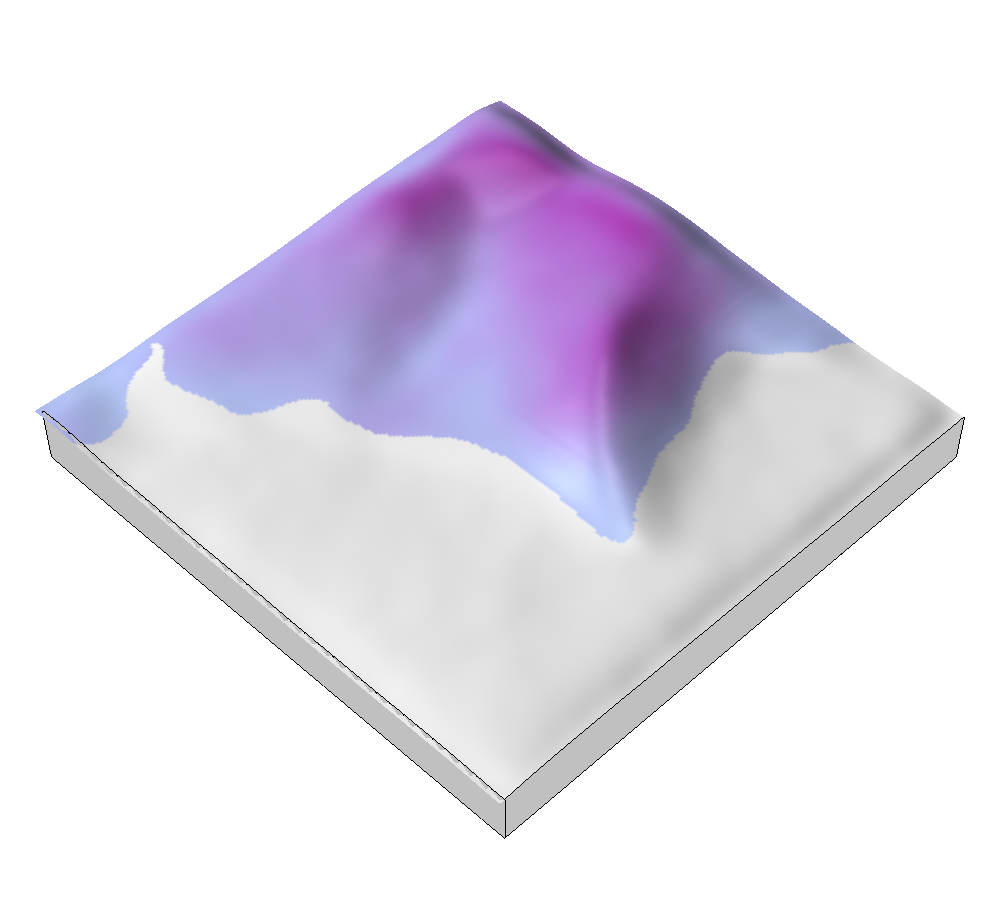
\includegraphics[width=0.18\textwidth]{images/render_3d/participants/stdev_dem_3.png}\\
%
Stdev.~of difference \par \vspace{0.5em} 
\includegraphics[width=0.16\textwidth]{images/legends/stdev_diff_legend.pdf} & 
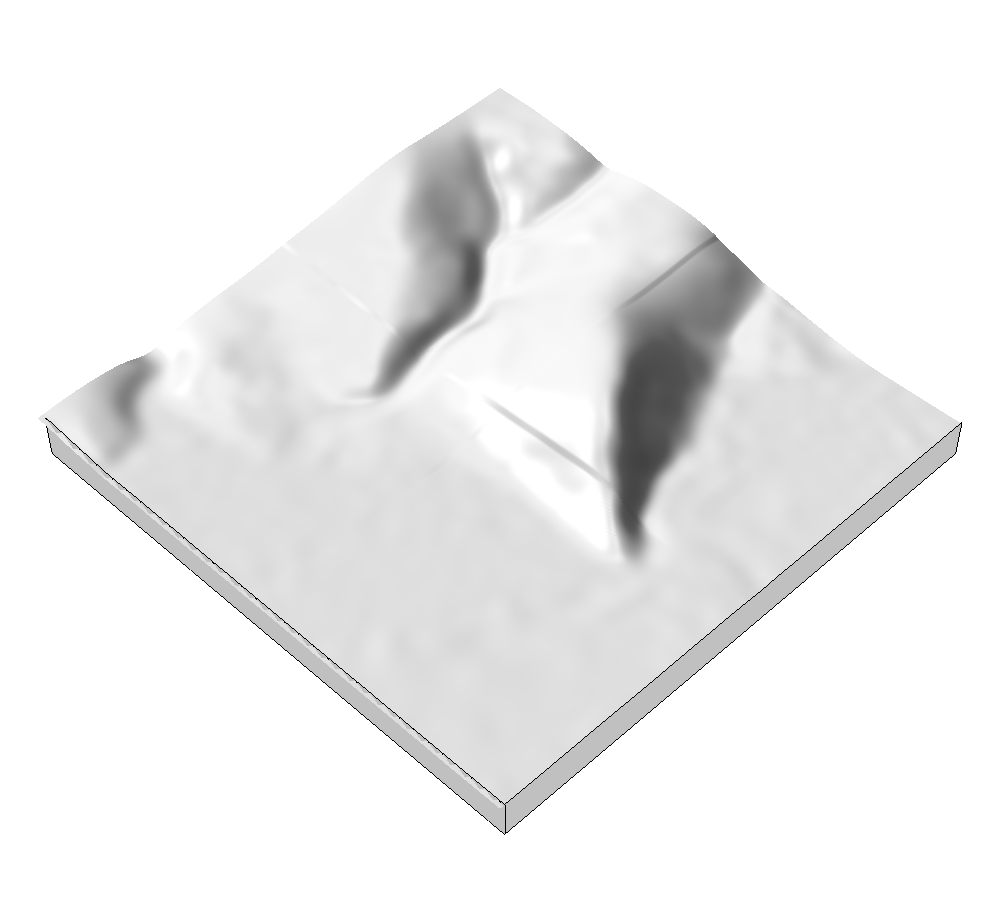
\includegraphics[width=0.18\textwidth]{images/render_3d/participants/dem_difference_1.png} &
\includegraphics[width=0.18\textwidth]{images/render_3d/participants/stdev_regression_difference_series_1.png} &
\includegraphics[width=0.18\textwidth]{images/render_3d/participants/stdev_regression_difference_series_2.png} &
\includegraphics[width=0.18\textwidth]{images/render_3d/participants/stdev_regression_difference_series_3.png}\\
%
Mean difference \par \vspace{0.5em} \includegraphics[width=0.16\textwidth]{images/legends/diff_legend.pdf} & 
\includegraphics[width=0.18\textwidth]{images/render_3d/participants/dem_difference_1.png} &
\includegraphics[width=0.18\textwidth]{images/render_3d/participants/mean_dem_regression_difference_1.png} &
\includegraphics[width=0.18\textwidth]{images/render_3d/participants/mean_dem_regression_difference_2.png} &
\includegraphics[width=0.18\textwidth]{images/render_3d/participants/mean_dem_regression_difference_3.png}\\
%
Mean slope \par \vspace{0.5em} \includegraphics[width=0.16\textwidth]{images/legends/slope_legend.pdf} & 
\includegraphics[width=0.18\textwidth]{images/render_3d/participants/slope_1.png} &
\includegraphics[width=0.18\textwidth]{images/render_3d/participants/mean_slope_1.png} &
\includegraphics[width=0.18\textwidth]{images/render_3d/participants/mean_slope_2.png} &
\includegraphics[width=0.18\textwidth]{images/render_3d/participants/mean_slope_3.png}\\
%
Mean landforms \par \vspace{0.5em} \includegraphics[width=0.16\textwidth]{images/legends/forms_legend.pdf} & 
\includegraphics[width=0.18\textwidth]{images/render_3d/participants/forms_1.png} &
\includegraphics[width=0.18\textwidth]{images/render_3d/participants/mean_forms_1.png} &
\includegraphics[width=0.18\textwidth]{images/render_3d/participants/mean_forms_2.png} &
\includegraphics[width=0.18\textwidth]{images/render_3d/participants/mean_forms_3.png}\\
%
\bottomrule
\end{tabular}
\label{table:topography}
%
\vspace*{1.5em}
%
\caption{Landforms identified by \textit{r.geomorphon} in Table~\ref{table:topography}:
		1)~flat, 
		2)~peak, 
		3)~ridge, 
		4)~shoulder, 
		5)~spur, 
		6)~slope, 
		7)~hollow, 
		8)~footslope, 
		9)~valley, and
		10)~depression.
		Source: \cite{r.geomorphon,Jasiewicz2013}}
\vspace*{1em}
\ra{1.3}
\begin{tabular}{m{0.6\textwidth}}
\includegraphics[width=0.6\textwidth]{images/geomorphons_legend.png}\\
\end{tabular}
\label{fig:geomorphons}
%
\end{table*}


% ---------------------------- CUT-FILL ---------------------------- 
\section{Cut-and-fill analysis}
% grading
When `grading' or earthmoving
landscape architects and civil engineers
seek to balance their sediment budget 
-- using as much cut (earth removed) 
as fill (earth deposited) --
to minimize the cost of transporting sediment 
to and from construction sites.
% difference method
Because of the importance 
of balancing sediment budgets
we designed a real-time analytic 
for Tangible Landscape that 
maps the difference in elevation
before and after modification
to assess topographic change and
facilitate cut-and-fill analysis. 
% experiment
To test the effectiveness of this real-time analytic
we conducted a cut-and-fill experiment.

\subsection{Methods}
In the cut-and-fill experiment 
the same 18 participants were asked to use 
Tangible Landscape's difference analytic to model 
another study landscape
with a large central ridge 
flanked by valleys 
and a smaller, secondary ridge.
Participants had 10 minutes to model this region
in polymer-enriched sand using Tangible Landscape 
with the difference analytic (Table~\ref{fig:diff}). 
The difference between the reference elevation 
and the participant's modeled elevation
was computed in near real-time and projected onto the sand 
as an interactive guide.
The linear regression of the reference and scanned elevation maps 
was used to correct shifts in scanning and georeferencing. 
The difference showed where 
sand needs to added (blue) or removed (red) 
in order to match the reference landscape.
% video
See \url{https://youtu.be/Q3elMIRCYSk}
for a video demonstrating the 3D modeling task 
with the difference analytic.

\paragraph{Data collection and analysis}
The final scan of each model was stored in a 
GRASS GIS database for analysis. 
We used raster statistics, the difference in elevation, 
topographic parameters, and morphometric parameters
to compare the reference elevation 
and the set of modeled elevations. 
We computed 
the mean elevation,
the standard deviation of elevations, 
and the standard deviation of difference for the set.
To find the standard deviation of differences 
we first computed the difference 
between the reference elevation and each elevation 
and then used raster statistics 
to calculate the standard deviation of these differences.
We also computed the difference between the 
reference elevation and the mean elevation for the set. 
The reference elevation used in the difference calculation 
was rescaled and shifted based on the 
linear regression of the reference and mean elevation.
We computed the slope and landforms of the mean elevation. 
We also filmed each session, 
observed and took notes on participants' modeling processes, 
and interviewed participants.

\subsection{Results}
% table
The 3D maps of raster statistics and geospatial analyses in
Tables~\ref{table:difference_comparison}-\ref{table:difference_percent_cells} 
show how participants performed with the difference analytic.
% overview of results
Participants performed well with the difference analytic 
-- modeling simplified, 
but relatively accurate approximations of the landscape.
Participants with expertise in 3D modeling 
performed even better than other participants 
-- more accurately modeling the elevation and slopes,
but not the landforms. 
Since these models were sculpted in sand,
their edges tend to slump.
This caused systematic artifacts in the analysis like
low elevation values and steep slopes
along the borders. 
Based on interviews and observations
we found that the difference analytic enabled
a rapid, iterative process 
of modeling, learning from computational feedback, 
re-remodeling, etc.

%  mean
The mean elevation modeled in this task
has the approximate shape of the reference elevation, 
but is much simpler, lacking many details. 
% stdev diff
The standard deviation of difference shows 
how consistently the models fit the reference. 
Overall participants performed well -- 
there was little deviation from the best fit. 
Participants tended to perform poorly 
near the edges of models, especially in the corners.
They also had trouble with the valleys 
and the low point by the secondary ridge.
% slope
The mean slope shows that participants tended to model 
overly steep slopes for the primary ridge -- exaggerating its form --
but tended not model steep enough slopes for the secondary ridge. 
% landforms
The mean landforms show that participants tended to 
clearly capture the central ridge and its spurs and
the secondary ridge and its valley, but missed the 
other valleys.
Hollows -- transitions between slopes, footslopes, and valleys -- 
on the mean landform map hint at these other 
valleys in the right locations.
% experts
The 3D modeling experts built more accurate models
with a lower standard deviation of differences 
and more accurate slopes. 
Since they did not, however, exaggerate the central ridge
and did not smooth its slopes, 
they did not cleanly represent this landform. 
The others built more exaggerated models 
that more clearly captured the main ridge.

% understanding volume
To successfully use the difference analytic 
participants had to think about topography as volume.
They had to either add or excavate sand to make the models match. 
One of the participants 
described modeling with the difference analytic
as a continual process of 'rebuilding to make it match.'
% iterative process
When interviewed
participants described an iterative process of 
continual refinement based on critical analysis 
-- similar to Sch{\"o}n's reflection-in-action \cite{Schon1983} --
but enhanced by computational feedback,
explaining that 
`because Tangible Landscape gives immediate results, 
it encourages an iterative process.' 
See Table \ref{table:interviews} for select comments about this experiment.

% conclusions
The difference analytic is intuitive -- 
participants were able to learn how to use it effectively without training, 
producing good, albeit exaggerated approximations of the landscape. 
%
Their models tended to have key morphometric characteristics -- 
the primary ridge, its spurs, the low point, 
the secondary ridge, and one of the valleys -- 
but these characteristics tended to be 
either over- or under-exaggerated.

% ---------------------------- DIFFERENCE ---------------------------- 

\begin{table*}[h]
\small\sf\centering
%
\caption{Cut-and-fill experiment: a participant sculpts the study landscape using Tangible Landscape's difference analytic, which shows where to add sand (blue) and remove sand (red).}
\vspace*{1em}
\ra{1.3}
\begin{tabular}{m{0.425\textwidth} m{0.425\textwidth}}
\includegraphics[width=0.425\textwidth]{images/experiments/difference_1.jpg} &
\includegraphics[width=0.425\textwidth]{images/experiments/difference_2.jpg}\\
\end{tabular}
\label{fig:diff} 
%
\vspace*{1.5em}
%
\caption{Cut-and-fill experiment: maps of raster statistics and geospatial analyses draped over a 3D rendering of the topography for all participants, 3D modeling novices, and 3D modeling experts.}
\vspace*{1em}
\ra{1.3}
\begin{tabular}{m{0.1\textwidth} m{0.2\textwidth} m{0.2\textwidth} m{0.2\textwidth} m{0.2\textwidth}}
\toprule
& \multicolumn{1}{c}{Elevation} & \multicolumn{1}{c}{Stdev.~ of differences} & \multicolumn{1}{c}{Slope} & \multicolumn{1}{c}{Landforms}\\
\midrule
%
Reference & 
\includegraphics[width=0.2\textwidth]{images/render_3d/3d_experts/dem_4.png} &
\includegraphics[width=0.2\textwidth]{images/render_3d/3d_experts/dem_difference_4.png}
&
\includegraphics[width=0.2\textwidth]{images/render_3d/3d_experts/slope_4.png} &
\includegraphics[width=0.2\textwidth]{images/render_3d/3d_experts/forms_4.png}\\
%
Mean & 
\includegraphics[width=0.2\textwidth]{images/render_3d/participants/mean_dem_4.png} &
\includegraphics[width=0.2\textwidth]{images/render_3d/participants/stdev_regression_difference_series_4.png} &
\includegraphics[width=0.2\textwidth]{images/render_3d/participants/mean_slope_4.png} &
\includegraphics[width=0.2\textwidth]{images/render_3d/participants/mean_forms_4.png}\\
%
3D novices & 
\includegraphics[width=0.2\textwidth]{images/render_3d/3d_novices/mean_dem_4.png} &
\includegraphics[width=0.2\textwidth]{images/render_3d/3d_novices/stdev_regression_difference_series_4.png} &
\includegraphics[width=0.2\textwidth]{images/render_3d/3d_novices/mean_slope_4.png} &
\includegraphics[width=0.2\textwidth]{images/render_3d/3d_novices/mean_forms_4.png}\\
%
3D experts & 
\includegraphics[width=0.2\textwidth]{images/render_3d/3d_experts/mean_dem_4.png} &
\includegraphics[width=0.2\textwidth]{images/render_3d/3d_experts/stdev_regression_difference_series_4.png} &
\includegraphics[width=0.2\textwidth]{images/render_3d/3d_experts/mean_slope_4.png} &
\includegraphics[width=0.2\textwidth]{images/render_3d/3d_experts/mean_forms_4.png}\\
%
& 
\multicolumn{1}{c}{\includegraphics[width=0.2\textwidth]{images/legends/elevation_legend_4.pdf}} &
\multicolumn{1}{c}{\includegraphics[width=0.2\textwidth]{images/legends/stdev_diff_legend.pdf}} &
\multicolumn{1}{c}{\includegraphics[width=0.2\textwidth]{images/legends/slope_legend.pdf}} &
\multicolumn{1}{c}{\includegraphics[width=0.2\textwidth]{images/legends/forms_legend.pdf}}\\
%
\bottomrule
\end{tabular}
\label{table:difference_comparison}
%
\vspace*{1.5em}
%
\caption{Cut-and-fill experiment: percent cells.}
\ra{1.3}
\begin{tabularx}{\textwidth}{YYYYYYYYYY}\toprule
Method && \multicolumn{2}{c}{Concentrated flow} & \phantom{abc}& \multicolumn{2}{c}{Ridges} &
\phantom{abc} & \multicolumn{2}{c}{Valleys}\\
\cmidrule{3-4} \cmidrule{6-7} \cmidrule{9-10}
&& Reference & Mean && Reference & Mean && Reference & Mean\\ \midrule
Difference && 1.94 & 0.90 && 4.27 & 2.93 && 2.96 & 0.13\\
\bottomrule
\end{tabularx}
\label{table:difference_percent_cells} 
%
\end{table*}


% ---------------------------- WATER FLOW ---------------------------- 
\section{Water flow modeling}

% importance of modeling water flow
Water, like earth, is another key medium of landscape architecture.
It can be challenging to understand, much less intentionally direct
the flow of water because this process
unfolds in time and space, 
driven by gravity and momentum and
controlled by the morphological shape and gradient of topography.
% simulation
We implemented a real-time water flow simulation 
for Tangible Landscape 
so that users can sculpt topography 
and immediately see how that changes 
the simulated flow and dispersion of water
across the landscape.
% experiment
After a pilot study \cite{Harmon2016}
we conducted an experiment to study 
how effectively landscape architects
can use this real-time, tangible water flow simulation.
% form and process
This experiment was designed to study whether
participants could link form and process
using the water flow simulation -- to assess
how well they could understand the relationship 
between topographic form 
and the flow of water 
when using Tangible Landscape.

\subsection{Methods}
The same 18 participants were asked to model water flow 
across another study landscape
using Tangible Landscape 
with the real-time water flow simulation 
(Table~\ref{fig:flow_sequence}).
This study region has a central ridge 
flanked by a large stream on one side 
and a small stream on the other.  
A third, smaller stream bisects the ridge.
Participants had 10 minutes to model water flow across this region.
Using Tangible Landscape
they sculpted polymer-enriched sand models of the topography
to direct the simulated flow of water.  
Water flow was simulated in near real-time 
as a diffusive wave approximation of shallow water flow.
The module \textit{r.sim.water} \cite{r.sim.water}
uses a path sampling technique to solve 
the shallow water flow continuity equation. \cite{Mitasova2004}
Participants could switch between 
the precomputed reference water flow -- i.e.~their target -- 
and the water flow over their scanned model.
% video
See \url{https://youtu.be/61hsXgb3MLY}
for a video demonstrating the 3D modeling task 
with the water flow simulation.

\paragraph{Data collection and analysis}
The final scan of each model was stored 
in a GRASS GIS database for analysis. 
We used raster statistics, simulated water flow, 
and the difference in simulated water depth 
to compare water flow across the study landscape 
and the set of models.
We computed the mean elevation,
the standard deviation of elevations, 
and the standard deviation of difference for the set.
Then we simulated water flow across 
the mean elevation for the set of models
and computed the difference 
between the reference and mean water flow. 

\subsection{Results}
% table
The 3D maps of raster statistics and geospatial simulations in
Table~\ref{table:water_flow_experiment} 
show how participants performed with the water flow simulation.
% overview of results
While all participants performed well in this task
-- typically capturing two of the three streams -- 
participants with expertise in 3D modeling performed the best.
These experts built more accurate models
that captured all three streams.

% mean elevation
The mean elevation modeled in this task
has under-exaggerated valleys and 
over-exaggerated ridges. 
The mean elevation has 22.43\% less valley cells 
than the reference, 
but 153.40\% more ridge cells
(see Table \ref{table:water_flow_percent_cells}). 
% stdev diff
The standard deviation of difference 
shows that participants performed well. 
The greatest deviation from the reference
was in the corners and along the edges
where the sand slumped.
% water depth
The mean water depth map shows two of the streams 
and hints of the third.
The streams are simplified, but in the right locations. 
The simplified stream channels lack micro-topography
and thus details. 
Table \ref{table:water_flow_percent_cells} shows that 
there was substantial concentrated flow (water depth $>=0.05$ ft) 
in the streams, albeit 31.10\% less than in the reference.
This is to be expected since 
water flow over the sculpted models 
was only computed over the model region, while 
the reference water flow 
was computed over a larger region 
with the entire contributing watershed 
in order to produce an accurate representation 
of water flow across the study landscape. 
% depth difference
The water depth difference map shows
where there should be more (red) or less (blue) water
to match the reference
-- i.e.~where water should flow versus where it was modeled. 
The mean water flow tightly fits the reference, 
following similar, albeit simplified routes.

% observations
With the tangible water flow simulation
participants focused on accurately modeling the streams, 
rather than the general shape of the topography. 
As a result the primary ridge was 
inconsistently modeled and over-exaggerated,
while the streams consistently 
had continuous, concentrated flow 
along the correct routes.
% understanding water flow
This experiment required abstract spatial thinking linking form and process. 
Because water flow is controlled by the shape and gradient of the topography
participants had to sculpt topographic form to drive water flow. 
% interviews
This modeling process, however, helped them understand topography better 
because `seeing the flow took away the mystery of topography.'
%
We observed participants using an iterative modeling process 
with the water flow simulation -- 
they 
\begin{enumerate*}[label=\alph*),font=\itshape]
\item sculpted the topography, 
\item observed how the water flow simulation changed, 
\item critiqued their water flow and topographic forms, 
\item and continued to sculpt.
\end{enumerate*}
%
Through this simulation-driven trial-and-error process 
participants were able 
to generate hypotheses, test hypotheses, and draw inferences 
about the way that water flows over topography. 
See Table \ref{table:interviews} for select comments about this experiment.

% ---------------------------- WATER FLOW ---------------------------- 

\begin{table*}[H]
\small\sf\centering
%
\caption{Water flow experiment: a participant sculpts the study landscape using Tangible Landscape's water flow analytic.}
\vspace*{1em}
\ra{1.3}
\begin{tabular}{m{0.5\textwidth}}
\includegraphics[width=0.5\textwidth]{images/experiments/tl_water.jpg}\\
\end{tabular}
\label{fig:flow_sequence} 
%
\vspace*{1.5em}
%
\caption{Water flow experiment: maps of raster statistics and geospatial analyses draped over a 3D rendering of the topography for all participants, 3D modeling novices, and 3D experts.}
\vspace*{1em}
\ra{1.3}
\begin{tabular}{m{0.1\textwidth} m{0.2\textwidth} m{0.2\textwidth} m{0.2\textwidth} m{0.2\textwidth}}
\toprule
& \multicolumn{1}{c}{Elevation} & \multicolumn{1}{c}{Stdev.~ of differences} & \multicolumn{1}{c}{Water depth} & \multicolumn{1}{c}{Depth difference}\\
\midrule
%
Reference & 
\includegraphics[width=0.2\textwidth]{images/render_3d/3d_experts/dem_5.png} &
\includegraphics[width=0.2\textwidth]{images/render_3d/3d_experts/dem_difference_5.png}
&
\includegraphics[width=0.2\textwidth]{images/render_3d/3d_experts/depth_5.png} &
\includegraphics[width=0.2\textwidth]{images/render_3d/3d_experts/dem_difference_5.png}\\
%
Mean & 
\includegraphics[width=0.2\textwidth]{images/render_3d/participants/mean_dem_5.png} &
\includegraphics[width=0.2\textwidth]{images/render_3d/participants/stdev_regression_difference_series_5.png} &
\includegraphics[width=0.2\textwidth]{images/render_3d/participants/mean_depth_5.png} &
\includegraphics[width=0.2\textwidth]{images/render_3d/participants/mean_depth_difference_5.png}\\
%
3D novices & 
\includegraphics[width=0.2\textwidth]{images/render_3d/3d_novices/mean_dem_5.png} &
\includegraphics[width=0.2\textwidth]{images/render_3d/3d_novices/stdev_regression_difference_series_5.png} &
\includegraphics[width=0.2\textwidth]{images/render_3d/3d_novices/mean_depth_5.png} &
\includegraphics[width=0.2\textwidth]{images/render_3d/3d_novices/mean_depth_difference_5.png}\\
%
3D experts & 
\includegraphics[width=0.2\textwidth]{images/render_3d/3d_experts/mean_dem_5.png} &
\includegraphics[width=0.2\textwidth]{images/render_3d/3d_experts/stdev_regression_difference_series_5.png} &
\includegraphics[width=0.2\textwidth]{images/render_3d/3d_experts/mean_depth_5.png} &
\includegraphics[width=0.2\textwidth]{images/render_3d/3d_experts/mean_depth_difference_5.png}\\
%
& 
\multicolumn{1}{c}{\includegraphics[width=0.2\textwidth]{images/legends/elevation_legend_5.pdf}} &
\multicolumn{1}{c}{\includegraphics[width=0.2\textwidth]{images/legends/stdev_diff_legend.pdf}} &
\multicolumn{1}{c}{\includegraphics[width=0.2\textwidth]{images/legends/depth_legend.pdf}} &
\multicolumn{1}{c}{\includegraphics[width=0.2\textwidth]{images/legends/depth_diff_legend.pdf}}\\
%
\bottomrule
\end{tabular}
\label{table:water_flow_experiment} 
%
\vspace*{1.5em}
%
\caption{Water flow experiment: percent cells.}
\ra{1.3}
\begin{tabularx}{\textwidth}{YYYYYYYYYY}\toprule
Method && \multicolumn{2}{c}{Concentrated flow} & \phantom{abc}& \multicolumn{2}{c}{Ridges} &
\phantom{abc} & \multicolumn{2}{c}{Valleys}\\
\cmidrule{3-4} \cmidrule{6-7} \cmidrule{9-10}
&& Reference & Mean && Reference & Mean && Reference & Mean\\ \midrule
\mbox{Water flow} && 3.28 & 2.26 && 1.18 & 2.99 && 4.77 & 3.70\\
\bottomrule
\end{tabularx}
\label{table:water_flow_percent_cells} 
\end{table*}


\begin{table*}
\caption{Interviews}
\ra{1.75}
\begin{tabular}{p{0.1\textwidth} p{ 0.85\textwidth}}
\toprule
Technology & Select comments\\
\midrule
%
Digital
%
& Rhino has a long learning curve.\\
& Understanding how Rhino works 
-- i.e.~the underlying mathematical representation, NURBS -- is very important. 
Once you understand that this surface is a tension field 
then you understand how to shape it, how to make it do what you want.\\
%
Analog 
%
& I worked additively, then subtractively, smoothing.
The sculpting tool gave sharpness --
the sharp edge let me smooth in a way my fingers couldn't.
It felt like drawing or laying concrete.
Feeling is important -- I could feel subtle changes in topography.\\
& My sense of touch helped me to understand the topography.
I could sculpt like reading braille. I could feel the shape with my fingers.
It was intuitive and calming.\\
%& I have done lots of sculpture so
%I knew how to feel the shape of the model. 
%And the desk lamp cast shadows so I could visually perceive depth.\\
%
Tangible
% 
%& We all already understand how sand works. 
%We understand sand, but not necessarily these analytics 
%-- the difference analytic or the water flow simulation.\\
& The difference analytic was the best. 
I tried to make it match. 
I was constantly rebuilding to make it match.
The water flow simulation was useful for thinking about form, 
about what form does --  why water flows where it does.
Seeing the flow takes away the mystery of topography.
Our students tend to have a linear design process.
Because Tangible Landscape gives immediate results 
it encourages an iterative process. \\
%& The water flow simulation reminds of me of playing 
%in creeks and grading streams as a kid.\\
& Tangible Landscape let me tinker. 
I could rapidly create, making new iterations. 
I could try something, see and feel it -- directly experience it --
and try again. Reinvent it.
Tinkering like this is a learning process. Learning through doing.
Tangible Landscape lowers the stakes so that you're not too invested.
You're ready to fail. So you can intuitively explore, 
while reflecting on what you've done,
what you're doing.\\
%
\bottomrule
\end{tabular}
\label{table:interviews}
\end{table*}

% ---------------------------- DISCUSSION ---------------------------- 
\section{Discussion}
% topographic
The topographic modeling experiment
shows that tangible modeling was 
more effective than either digital or analog sculpting. 
Tangible modeling was intuitive;
even the novices performed well without training or experience.
Drawing on embodied cognition
they were able to feel the 3D shape of their model
and knew automatically, subconsciously what to do --
how to shape it with their hands.
Intuitive interaction mattered less for the 3D modeling experts
because they had already acquired the knowledge and skills needed.
They still performed better with tangible modeling
because they were able to 
work faster and refine their models earlier. 

% cut-fill
In cut-and-fill experiment we found that
participants used an iterative modeling process
successfully combining the affordances of hand sculpting
with real-time geospatial analytics. 
Participants performed well without training; 
they managed to quickly learn and 
understand the analytic
and successfully used it to adaptively sculpt
accurate models.
This suggests that they were able to offload the cognitive work 
of manipulation onto their bodies, while cognitively 
parsing a rapidly changing, graphical representation 
of the difference in volume.

% water flow
The water flow experiment shows 
that the water flow simulation helped participants 
understand the relationship between form and process.
We observed participants using an iterative process
to adaptively sculpt based on the simulated water flow. 
Through this trial and error process 
participants learned how
topographic form controls the flow of water.
Given that they accurately represented the streams without training
they must have been able to offload 
some of the cognitive work of sensing and manipulating 
3D form onto their bodies so that 
they could focus on the water flow. 

% 3D expertise
The 3D modeling experts 
performed better than all other participants
including other experienced academics and professionals. 
First of all this shows that 
tangible modeling
can be effective for experts as well as novices. 
It also suggests that advanced spatial abilities and skills
developed with digital tools can be transferred
to tangible interfaces. 
If these abilities are transferable, 
then tangible interfaces 
-- given their intuitive, embodied nature --
may be a fast and effective way to train them.

\subsection{Open science} 
As a work of open science we invite readers to
replicate or build upon this experiment by 
using or adapting our tangible interface, 
experimental methodology, code, and data. 
%
See the supplemental material 
for links to the
code,
data and results, 
project website,
and videos.
%
The python scripts for data processing and analysis 
and the Tangible Landscape source code 
are released under the GNU General Public License (GPL).
All results related to this study 
-- including data, renderings, photographs, and interview notes --
are released under the Creative Commons Zero license
and linked in the supplemental material.

%The python scripts for data processing and analysis are 
%on GitHub at \url{https://github.com/baharmon/tangible_topography}
%released under the GNU General Public License (GPL).
%The data used in this experiment 
%and the results -- 
%including data, renderings, photographs, and interview notes -- are 
%on the Open Science Framework 
%at \url{https://osf.io/82gst/} under the Creative Commons Zero license.
%
%
%%build-your-own
%To build your own Tangible Landscape
%visit the project website at \url{http://tangible-landscape.github.io/}, 
%see the documentation in the GitHub repository 
%including the Wiki at \url{https://github.com/tangible-landscape/grass-tangible-landscape/wiki},
%and refer to the book Tangible Modeling with Open Source GIS. \cite{Petrasova2015}
%GRASS GIS is available at
%\url{https://grass.osgeo.org/} 
%under the GPL. 
%Tangible Landscape's components are available at
%\url{https://github.com/tangible-landscape}
%under the GPL. 

%\subsection{Future work}
%% improvements
%Based on these user studies and 
%our own reflections and experiences with Tangible Landscape
%we have identified ways to improve the system.  
%% what do users want?
%Our users want more tools that are natural to use 
%so that they can do whatever they imagine
%with their existing skills. 
%They want a richer, more immersive experience. 
%They want larger models and easier, faster, cheaper ways to build models.
%% refine existing modes of interaction 
%We plan to 
%refine existing modes of interaction 
%with new methods for handling, processing, and filtering point clouds.
%% new modes of interaction
%By fusing color and depth data
%we will develop new modes of interaction including
%planting individual trees of a given species with a model tree
%and building structures with building blocks. 
%% integration with 3D rendering
%We plan to support new VR headsets and integrate 
%procedural plant generation, 3D tree libraries, and 3D building libraries
%for more immersive renderings. 
%% larger models
%We plan to support arrays of multiple 3D sensors
%for scanning larger models.
%% better ways to build physical models 
%We plan to design better ways to build physical models
%using in-situ robotic fabrication. 
%% improved system setup
%We also plan to improve the system setup
%so that it is modular, lighter, more portable, more adaptable, less expensive,
%and more aesthetic.
%% future research
%We have also identified new research questions.
%How can Tangible Landscape be used effectively
%for other aspects of landscape architecture
%like planting design, ecological restoration, or landscape ecology?
%How can Tangible Landscape be used effectively 
%for participatory modeling and design?
%How can Tangible Landscape be used effectively in classrooms?

% ---------------------------- CONCLUSION ---------------------------- 

\section{Conclusion}
%
This study demonstrates that tangible landscape modeling
can be an effective design tool for landscape architects.
%
With systems like Tangible Landscape
landscape architects can naturally sketch or model in 3D,
while learning from real-time geospatial analytics.
%
As this study shows
landscape architects can
rapidly and accurately model topography, 
analyze topographic change, 
and direct the flow of water 
with Tangible Landscape.
%
They can work in a rapid, iterative design process,
quickly giving their ideas form and quantitatively testing them.

% design implications
With tangible modeling 
and real-time geospatial simulations 
landscape architects should be able design 
high performance, process-based landscapes.
%
Tangible modeling enables
the intuitive exploration and manipulation
of the complex interactions between 
geomorphological and ecological
form and process. 
%
By seamlessly integrating geospatial simulation into
the creative design process, 
physical processes like the flow of water and sediment
could play a generative role in landscape architecture. 

% ---------------------------- SUPPLEMENTAL MATERIAL ---------------------------- 

%https://us.sagepub.com/en-us/nam/supplementary-files-on-sage-journals-sj-guidelines-for-authors

\begin{sm}
%
\label{appendix:methodology}



% ---------------------------- TOPOGRAPHIC  ----------------------------
\section{Topographic modeling results}
\label{appendix:topographic_results}

% ALL PARTICIPANTS
\paragraph{All participants}
Tables \ref{table:coupling_experiment},
\ref{table:percent_cells}, 
and \ref{table:distance}
show the results for all participants. 
%
% DIGITAL
When digitally modeling with Rhino
participants were relatively 
consistent and accurate except in the interior space.
The interior space -- the main valley and the ridge -- 
tended to have serious errors.
%
They built very abstract massing models 
approximating the general shape of the landscape
without any detail. 
%
The slopes in these models 
were consistently too low and gradual.
They did not have enough curvature 
to create distinct landforms. 
%
These models only hinted at 
the morphology of landscape
with a small cluster of valley cells
and another small cluster of ridge cells.  
Key features like the stream channel
were not represented. 

% digital observations
We observed that most participants had trouble
judging depth and perceiving interior space 
when digitally modeling. 
We also observed most participants 
using similar digital modeling strategies 
in a relatively linear fashion.
Since the reference data -- the 3D contour curves -- 
clearly represented profiles, 
many participants first modeled
the borders of the landscape
relying heavily
on the front and side viewports.
Then in perspective view 
they began to pull up relative high points 
to build a rough massing model of the topography.
Finally they began to refine its shape 
by pulling down relative low points to 
steepen slopes and form valleys.
%
The 3D modeling experts, however, 
used unique modeling strategies
developing their own techniques as they worked.
One worked exclusively in the perspective viewport
continually orbited above and below the model 
in order to compare the top and the bottom
as he pushed and pulled points
in a very freeform, iterative process. 
%
Only the experts had time to rebuild the 
10 x 10 grid of control points as a 20 x 20 grid. 
This meant that all of the other models
had half the effective resolution
and were thus more approximate
representations of the landscape. 

% ANALOG
When sculpting by hand 
participants used very different modeling strategies 
and as a result they built very different models
as shown by the standard deviation of elevation.
While inconsistent, 
their models were relatively accurate
and captured the key landforms.
While they tended to over exaggerate the main ridge, 
they did represent
this ridge and most of the central valley.
Due to slumping sand
these models tended to be too low along the edges. 

% analog observations
We observed participants using 
a wide range of different modeling strategies
and techniques when sculpting by hand. 
They tended to work in a very freeform manner 
-- switching freely between
adding, removing, pressing, pushing, pulling, or smoothing
sand. 
% tool use
Some used only their bare hands, 
some used only the wooden sculpting tool,
and others used their bare hands to sculpt 
and the tool the refine details. 
% 3d scale use
Most participants used the 3D scale
to build highest point at the right height
-- some even buried the 3D scale in their model
building around it. 
%
Some participants instead 
picked up the reference model
and used its edges -- its profiles -- to build 
the sides of the model. 
Some participants also ran their fingers 
over the reference model to feel its shape.
A few  participants, however,
ignored both the 3D scale
and the reference model. 

We observed participants 
freely and rapidly switch between 
sculpting the sand with 
their whole hands,
their palms,
the blade of their hands, 
or just their fingertips 
depending on whether 
they wanted to make a big move
or a fine-tuned refinement.
%
While participants could select and transform
a group of control points in Rhinoceros,
their control was limited by the grid size, i.e. the number of points,
and their speed by the need to continually change the selection.
%
When we tested Vue as an alternative
with 3D painting and sculpting tools
with parameters like size and intensity
we found that these parameters 
required continually tuning,
which interrupted the modeling process 
and slowed down interaction.

% interviews
See Table \ref{table:interviews} for select comments from interviews.
One participant said that she felt anxious when digitally modeling,
but felt calmer and more relaxed when hand sculpting sand. 
She found hand sculpting to be more intuitive, saying that
while digital modeling had `a long learning curve,' 
she could read the sand model `like braille\ldots 
I could feel the shape with my fingers.'

% AUGMENTED
Overall participants performed best
with projection-augmented modeling
building more accurate models 
that represented the major landforms.
%
These models had the lowest mean minimum distance 
for cells with concentrated water flow, ridges, and valleys
(see Tables \ref{table:percent_cells} \& \ref{table:distance}). 
%
We observed participants using the same
modeling techniques, strategies, and tool use
as they did when sculpting by hand. 
They worked in the same freeform manner, but 
-- with the aid of the projected contours and elevation --
had more consistent results 
as shown by the standard deviation of elevations.
%
Overall, they had more accurate results
-- albeit with systemic errors along the borders 
due to slumping sand --
as shown by the mean difference and
standard deviation of differences. 
%
They correctly represented the main ridge and 
the central valley, but tended to miss details
like the y-shaped branch at the head of
of the stream channel. 

One participant found that 
with projection-augmented modeling 
he was able to effectively combine 
the affordances of hand sculpture 
with the extra layer of data. 
%
He described an iterative strategy of additive modeling
in which the projected `contours were just a guide' --  
`My general strategy was additive. 
I felt with my hands to try to match the contours. 
If I saw concavity in the contours 
then I felt the sand and sculpted that concavity.
Finding the relative height, however, was challenging -- 
it was subtle.'

\paragraph{Students vs. academics and professionals}
%
Table \ref{table:students} and Table \ref{table:professionals}
compare students' results 
with academics and professionals. 
% overview
Overall the academics and professionals
only performed slightly better than the students.
% digital
When digitally modeling both groups 
built very approximate massing models
that only hinted at the landforms. 
While the professionals and academics 
managed to create a small cluster of valleys cells
in the central stream channel, 
the students tended to miss this feature. 
% analog
When sculpting by hand
both groups' performance improved dramatically;
they built more accurate models
as shown by the standard deviation of difference
and better represented the landforms
roughly capturing the main ridge and valley. 
%
With projection augmented modeling
both groups' performance increased even more
as shown by the low standard deviation of difference.

\paragraph{Landscape architecture vs. GIS students}
%
Table \ref{table:landscape_students} and
Table \ref{table:gis_students}
compare landscape architecture and GIS students' results.
%
% overview
The GIS students built more abstract, approximate models
than the landscape architecture students who tended to 
over-exaggerate the shape of the landscape.
%
With each technology the GIS students' 
performance improved;
they built more and more accurate models 
with more distinct landforms.
The landscape architecture students' performance, however, 
did not improve significantly between
analog and projection-augmented modeling. 
% digital 
With digital modeling both groups
had major errors along the ridge,
but the GIS students also had serious problems
with the interior space.
The GIS students missed
the central valley entirely, while the landscape students
hinted at it with a small cluster of valley cells. 
%
When hand sculpting 
both groups made major improvements.
The GIS students began to form
the main ridge and valley. 
They tended to build too large a ridge
with the highest point near its tip
and significant errors on its slopes. 
The landscape architecture students tended to 
hand sculpt distorted, exaggerated landscapes 
with extras landforms, 
but roughly captured the y-shaped stream. 
%
With projection augmented modeling 
the GIS students captured
the central valley and ridge,
correctly modeled steeper slopes,
and had much less errors as shown by 
the standard deviation of difference.
%
The landscape architecture students, however,
did not make significant improvements 
over their hand sculpted models. 

\paragraph{Academics and professionals with and without 3D modeling expertise}
%
Table \ref{table:3d_novices} and Table \ref{table:3d_experts}
compare landscape architecture academics and professionals 
with and without 3D modeling expertise. 
% overview
While the other academics and professionals
performed poorly with digital modeling, 
better with analog modeling, 
and best with projection augmented modeling,
the expert 3D modelers built very accurate models
with each technology, but represented the landforms
best with projection augmented modeling.
% digital
While the rest of the academics and professionals 
had major errors on the ridge 
in the digital modeling task,
the expert 3D modelers built accurate models 
with very low mean difference and 
standard deviation of difference. 
The 3D experts worked faster
and had time to rebuild denser grids of control points
so that they could build more detailed,
higher resolution models.
Despite their accuracy their digitally sculpted models 
still only hinted at the landforms 
with small clusters of valley and ridge cells. 
% analog
The 3D modeling experts represented 
more complete landforms when sculpting by hand,
capturing details like the y-shaped branch of the stream,
but missed much of the ridge. 
% augmented
With projection augmented modeling 
the expert 3D modelers performed even better
successfully capturing
the ridge, the valley, and its y-shaped branch
with few anomalous features. 
%
They used the wooden modeling tool 
to cut clean edges around their models
minimizing systematic errors caused by slumping sand.

\noindent
Python scripts for data processing and analysis: \\
\noindent
\url{https://github.com/baharmon/tangible_topography}

\noindent
Data, results, and methods: \url{https://osf.io/82gst/}

\noindent
Website: \url{http://tangible-landscape.github.io/}

\noindent
GitHub: \url{https://github.com/tangible-landscape}

\noindent
Wiki: \url{https://github.com/tangible-landscape/grass-tangible-landscape/wiki}

\noindent
Videos: \url{youtube.com/c/NCSUGeoForAllLab}
%\end{sm}

% ------------------- INTERVIEW GUIDELINES ----------------------- 

\vspace*{1em}
%
\noindent \textbf{Semi-structured interview guidelines}\label{appendix:guidelines} \\

\textbf{Interview goals}
\begin{itemize}
\item Map participants' analog, hand modeling processes
\item Map participants' digital modeling processes
\item Map participants' tangible modeling processes
\item Map participants' tangible modeling processes with the cut-and-fill analytic
\item Map participants' tangible modeling processes with the water flow analytic
\end{itemize}

\textbf{\emph{Topic:} Modeling process}
\begin{itemize}
\item Please describe your modeling process with each technology
\item Did you work additively or subtractively? A mix?
\item Did you work in a linear or an iterative, exploratory process?
\item How did this technology aid you? What did it let you to do?
\item Did this technology constrain you in any way?
\end{itemize}

\textbf{\emph{Topic:} Intuition}
\begin{itemize}
\item How intuitive was it? 
\item Could you model what you intended?
\item Did you have to think about how to modeling? Or could you just act?
\end{itemize}

\textbf{\emph{Topic:} Metacognition}
\begin{itemize}
\item We asked you to sculpt a model of the study landscape. Please describe your thought process while sculpting. 
\item Did you strategize about how to model? If so what was your modeling strategy? 
\item Did your modeling strategy evolve as you worked?
\end{itemize}

\textbf{\emph{Topic:} perception and experience}
\begin{itemize}
\item How did it feel to sculpt a 3D model with this technology?
\item Was it stressful? Was it fun?
\item Did the technology change how you perceived distance, depth, form, or volume?  
\end{itemize}

\end{sm}


% ---------------------------- BIBLIOGRAPHY ---------------------------- 

\bibliographystyle{SageV}
\bibliography{tangible_topography.bib} 

\end{document}
